\documentclass[11pt,a4paper]{article}

\usepackage[a4paper,margin=22mm,headheight=15pt]{geometry}
\usepackage[T1]{fontenc}
\usepackage[utf8]{inputenc}
\usepackage{lmodern}
\usepackage{microtype}
\usepackage{graphicx}
\usepackage{float}
\usepackage{booktabs}
\usepackage{longtable}
\usepackage{array}
\usepackage{xcolor}
\usepackage{amsmath}
\usepackage{amssymb}
\usepackage{listings}
\usepackage{subcaption}
\usepackage{enumitem}
\usepackage{fancyhdr}
\usepackage[hidelinks]{hyperref}
\usepackage[most]{tcolorbox}
\usepackage{placeins}

\graphicspath{{figures/}}
\setlength{\parindent}{0pt}
\setlength{\parskip}{0.65em}
\renewcommand{\arraystretch}{1.16}
\setlist{itemsep=0.25em,topsep=0.3em}

\definecolor{navy}{HTML}{17324D}
\definecolor{teal}{HTML}{155E75}
\definecolor{softblue}{HTML}{EAF3F7}
\definecolor{softamber}{HTML}{FFF7E6}
\definecolor{softgrey}{HTML}{F3F4F6}
\definecolor{codegreen}{HTML}{166534}

\hypersetup{
  pdftitle={Communication Engineering Labbook -- Answered Questions and Evidence},
  pdfauthor={Aaron Taylor},
  colorlinks=true,
  linkcolor=navy,
  urlcolor=teal
}

\pagestyle{fancy}
\fancyhf{}
\lhead{ENEL700 Communication Engineering}
\rhead{Aaron Taylor}
\cfoot{\thepage}

\newtcolorbox{answerbox}{
  breakable,
  colback=softblue,
  colframe=teal,
  boxrule=0.7pt,
  arc=2mm,
  title=My answer,
  fonttitle=\bfseries
}

\newtcolorbox{evidencebox}{
  breakable,
  colback=softgrey,
  colframe=navy,
  boxrule=0.6pt,
  arc=2mm,
  title=Evidence boundary,
  fonttitle=\bfseries
}

\newtcolorbox{checkbox}{
  breakable,
  colback=softamber,
  colframe=orange!65!black,
  boxrule=0.6pt,
  arc=2mm,
  title=Preserved uncertainty,
  fonttitle=\bfseries
}

\lstdefinestyle{matlab}{
  language=Matlab,
  basicstyle=\ttfamily\small,
  keywordstyle=\color{blue!65!black}\bfseries,
  commentstyle=\color{codegreen},
  stringstyle=\color{red!60!black},
  numbers=left,
  numberstyle=\tiny\color{gray},
  stepnumber=1,
  numbersep=8pt,
  frame=single,
  rulecolor=\color{gray!40},
  breaklines=true,
  showstringspaces=false,
  backgroundcolor=\color{gray!4}
}

\title{\vspace{-1.5cm}\textbf{Communication Engineering Labbook}\\[0.3em]
\Large Answered Questions, Evidence and Graphs}
\author{Aaron Taylor\\ENEL700 Communication Engineering}
\date{2 August 2026}

\begin{document}
\maketitle

\begin{evidencebox}
I wrote this supplement in the first person from my running labbook and the files preserved in our in-class folders. I treat the in-class photographs, screenshots, model files and raw measurement transcription as the primary evidence of what my group actually did. I label later calculations and MATLAB replication separately. Where the surviving evidence does not answer a question, I say so rather than inventing a detail.
\end{evidencebox}

\tableofcontents
\newpage

\section{Direct answers to the open questions in my running labbook}

\subsection{Lab 5: amplitude modulation using Simulink}

\subsubsection*{What exact code or plotting change produced the three stacked spectra?}
\begin{answerbox}
The preserved files do not identify one decisive line as the final fix. What I can verify is the final working arrangement: I selected each axis with \texttt{subplot(3,1,k)} before calling \texttt{sigspec} for the modulating signal, carrier and modulated signal. I also had to keep the signals in compatible vector orientations and use the same spectrum function for all three. This produced three separate, vertically stacked spectra rather than repeatedly drawing into one axis. I should not claim a more specific last edit because I did not record it at the time.
\end{answerbox}

\subsubsection*{Did a lecturer or classmate identify the decisive fix?}
\begin{answerbox}
I did not preserve enough evidence to attribute the decisive plotting fix to a lecturer or classmate. My logbook records collaborative troubleshooting and several attempts, but it does not name a person who supplied the final correction. I therefore leave the attribution unclaimed.
\end{answerbox}

\subsubsection*{What did the final Scope show?}
\begin{answerbox}
Our saved model routed the Product output to a Scope, so the intended Scope result was an AM double-sideband suppressed-carrier waveform: a rapidly oscillating carrier whose positive and negative envelope followed the two-arch message. However, I did not preserve an identifiable in-class Scope capture. The strongest saved class result is the final three-spectrum screenshot below. I therefore use the Scope description as the expected interpretation of the model, not as a claim about a missing screenshot.
\end{answerbox}

\begin{figure}[H]
  \centering
  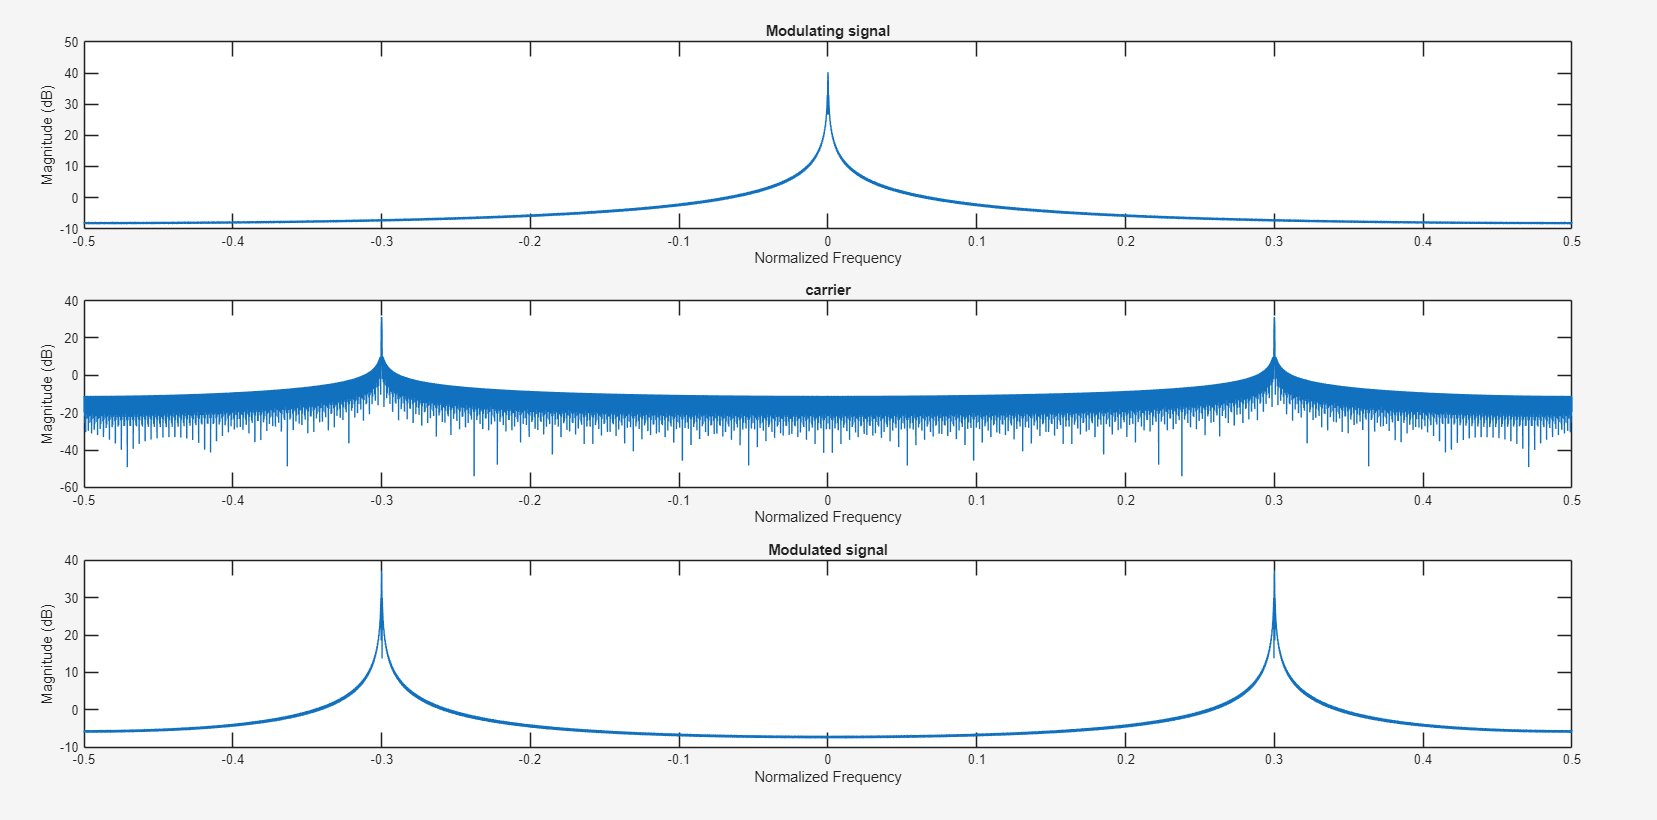
\includegraphics[width=0.96\textwidth]{lab5_inclass_spectra.png}
  \caption{Primary in-class evidence from Lab 5: our saved three-spectrum result. The baseband message is centred near zero, while the modulated spectrum is translated to the carrier regions near normalized frequency $\pm 0.3$.}
  \label{fig:lab5-class-spectra}
\end{figure}

\begin{figure}[H]
  \centering
  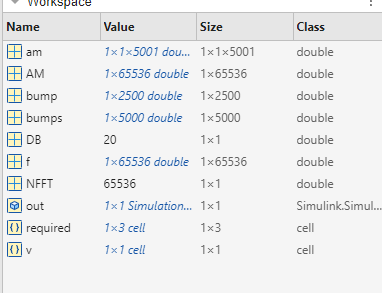
\includegraphics[width=0.48\textwidth]{lab5_workspace.png}
  \caption{Primary in-class MATLAB workspace evidence retained with our Lab 5 files.}
  \label{fig:lab5-workspace}
\end{figure}

\subsection{Lab 4: pulse-code modulation}

\subsubsection*{Who attended Lab 4 with me?}
\begin{answerbox}
Nahil attended Lab 4 with me. The other two group members were sick, so Nahil and I completed the class work as a pair. We first worked out how to read the four data-bit positions in the PCM frame, checked our interpretation with the lecturer and nearby classmates, and then divided the task between changing the input and recording each voltage/code pair.
\end{answerbox}

\subsubsection*{Are $-0.308$ V and $-0.270$ V exact values?}
\begin{answerbox}
They are the values preserved in my typed class-data transcription, but none of the retained meter photographs shows either value. I cannot independently confirm them from the surviving evidence. I have therefore plotted them exactly as recorded and highlighted them for checking rather than silently changing them. The $0.038$ V spacing between these adjacent codes is much smaller than the typical spacing in the rest of the linear table, so at least one of these entries may contain a transcription or measurement error.
\end{answerbox}

\subsubsection*{Were only 11 companded points measured?}
\begin{answerbox}
Only 11 companded points are preserved in the class-data file. The recorded decimal codes are 0, 1, 2, 3, 4, 9, 11, 12, 13, 14 and 15. Codes 5, 6, 7, 8 and 10 are absent. I found no second in-class table containing the missing values, so I describe the companded graph as partial rather than presenting it as a complete 16-level law.
\end{answerbox}

\subsubsection*{Can I confirm the evidence-photo grouping?}
\begin{answerbox}
Yes. The visible meter readings match the class-data table to within approximately 1 mV. The photographs at about $-2.634$, $-2.240$, $-1.911$ and $-1.595$ V match Question 4.1 codes 0000, 0001, 0010 and 0011. The photographs at about $-2.633$ and $-1.100$ V match Question 4.2 codes 0000 and 0001. Both photographs near $-2.63$ V show a minus sign; neither is evidence for the positive endpoint.
\end{answerbox}

\section{Lab 4 evidence and measured graphs}

\begin{figure}[H]
\centering
\begin{subfigure}[t]{0.48\textwidth}
  \centering
  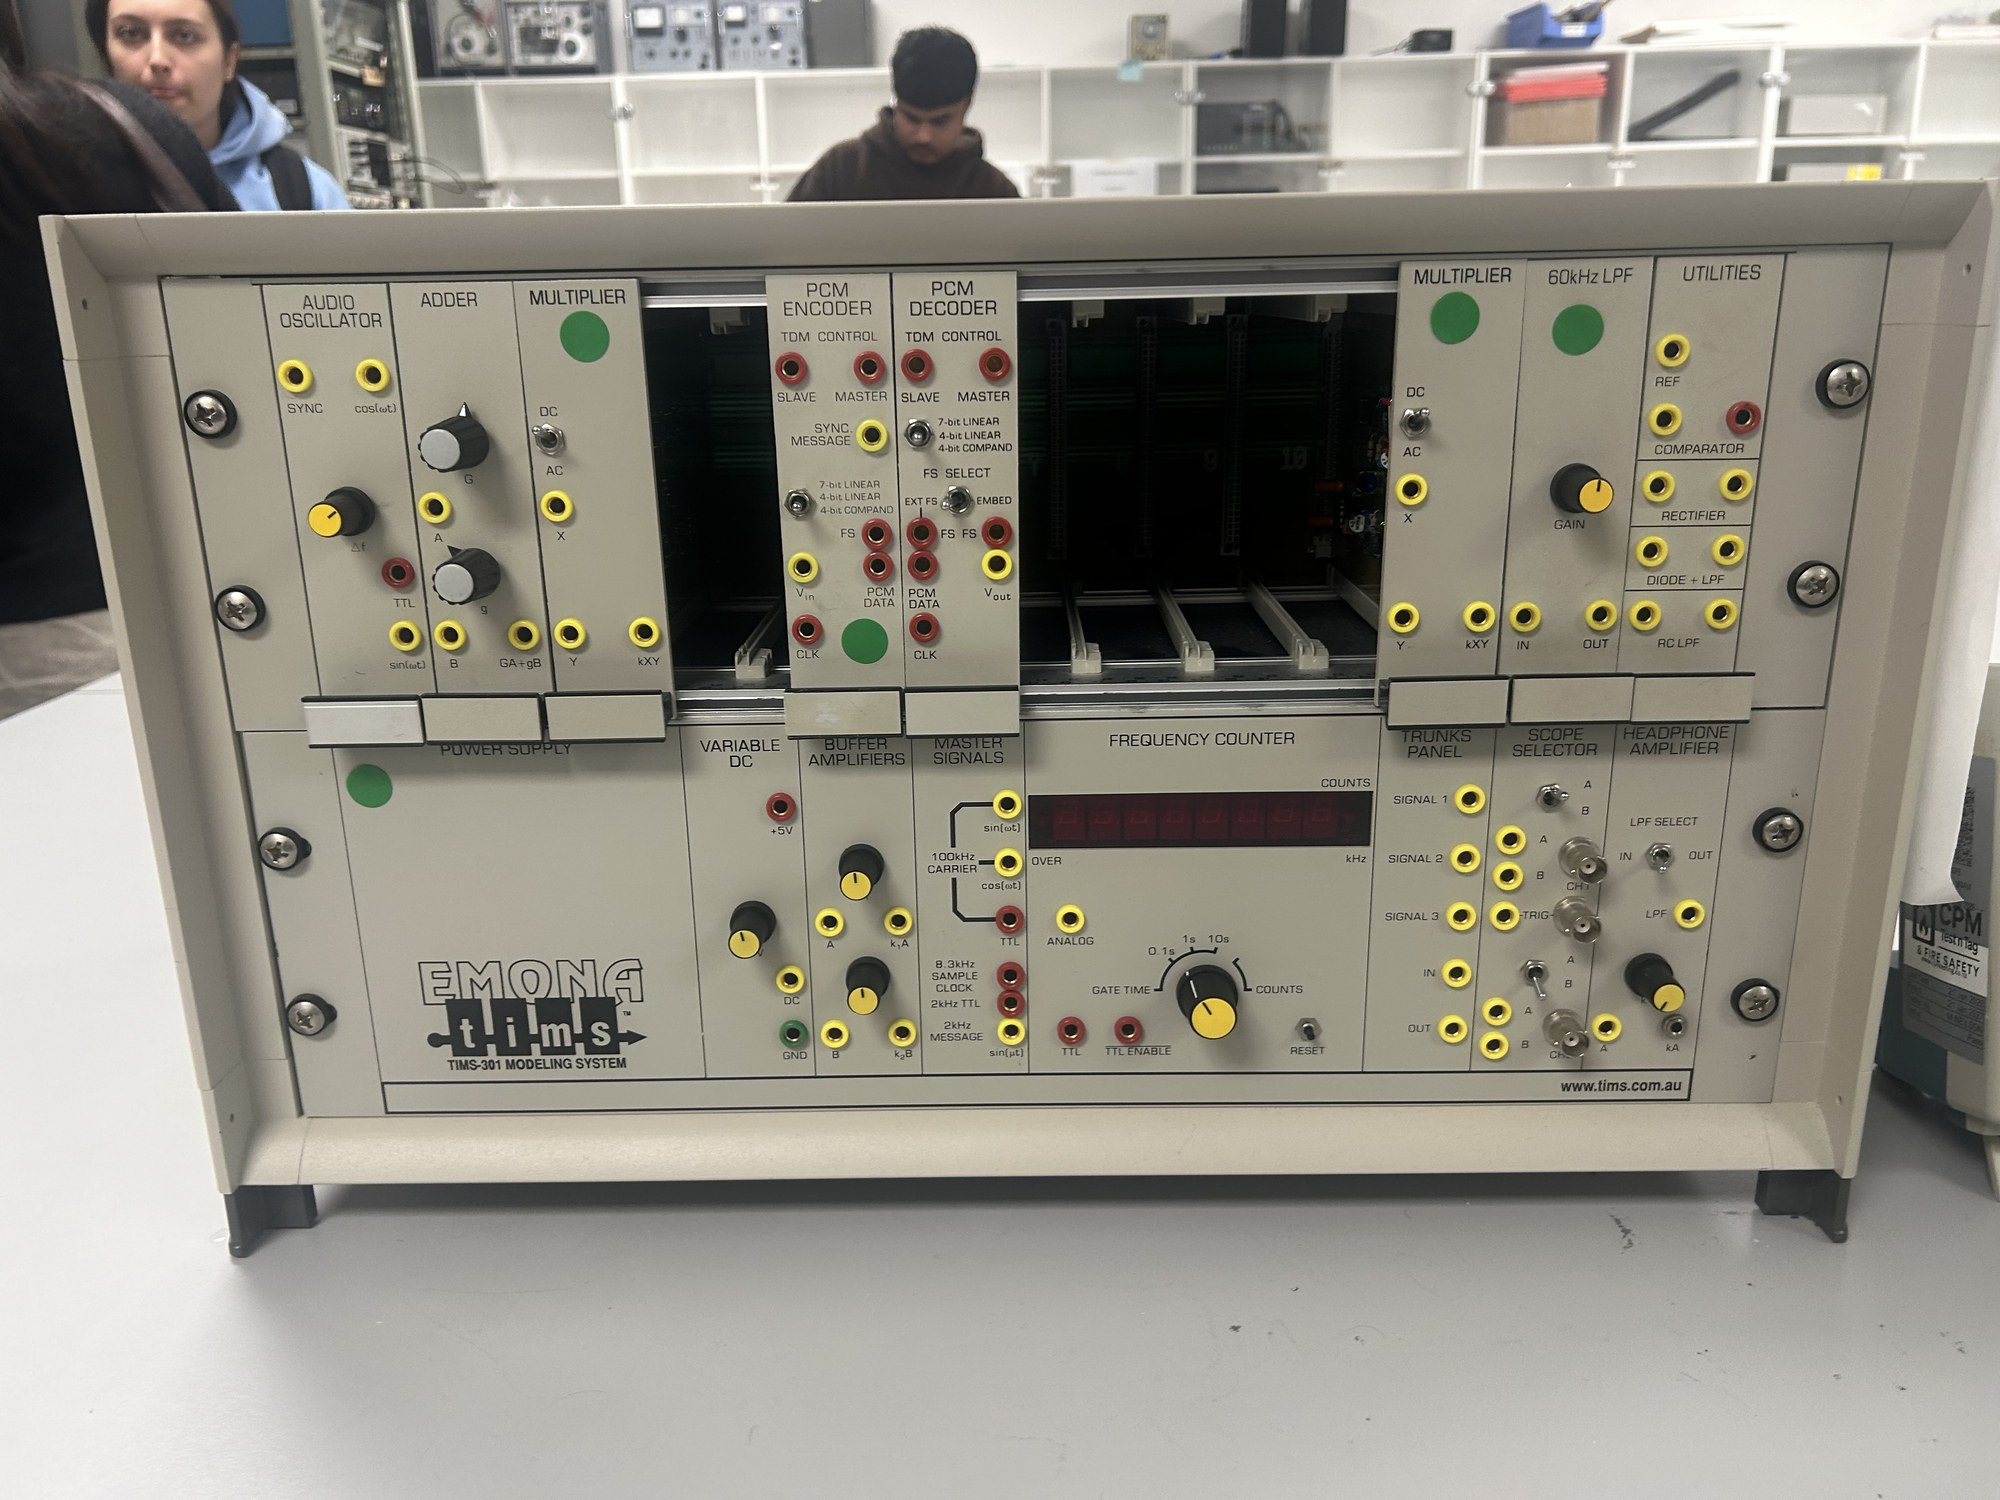
\includegraphics[width=\linewidth]{lab4_tims_system.jpg}
  \caption{The TIMS-301 system used in class.}
\end{subfigure}\hfill
\begin{subfigure}[t]{0.48\textwidth}
  \centering
  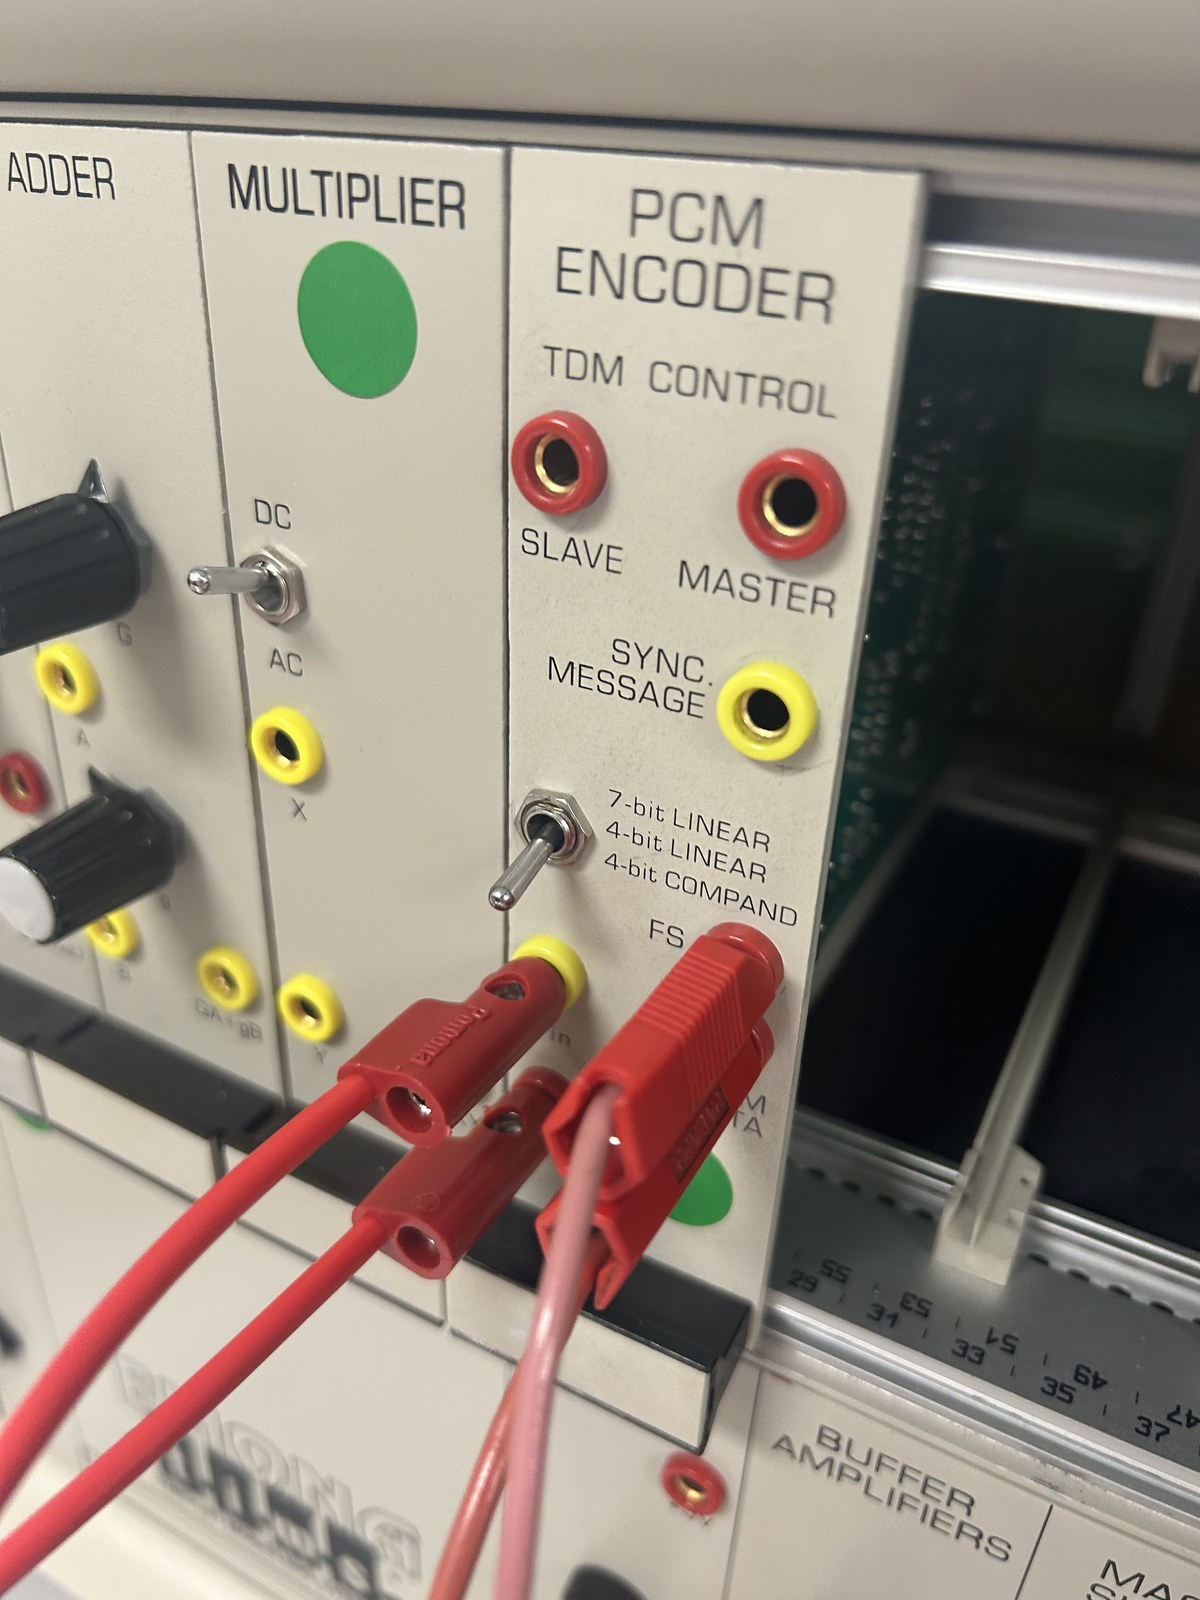
\includegraphics[width=\linewidth]{lab4_encoder_patch.jpg}
  \caption{Our in-class PCM encoder patching.}
\end{subfigure}
\caption{Primary physical evidence from Lab 4.}
\label{fig:lab4-setup}
\end{figure}

\begin{figure}[H]
  \centering
  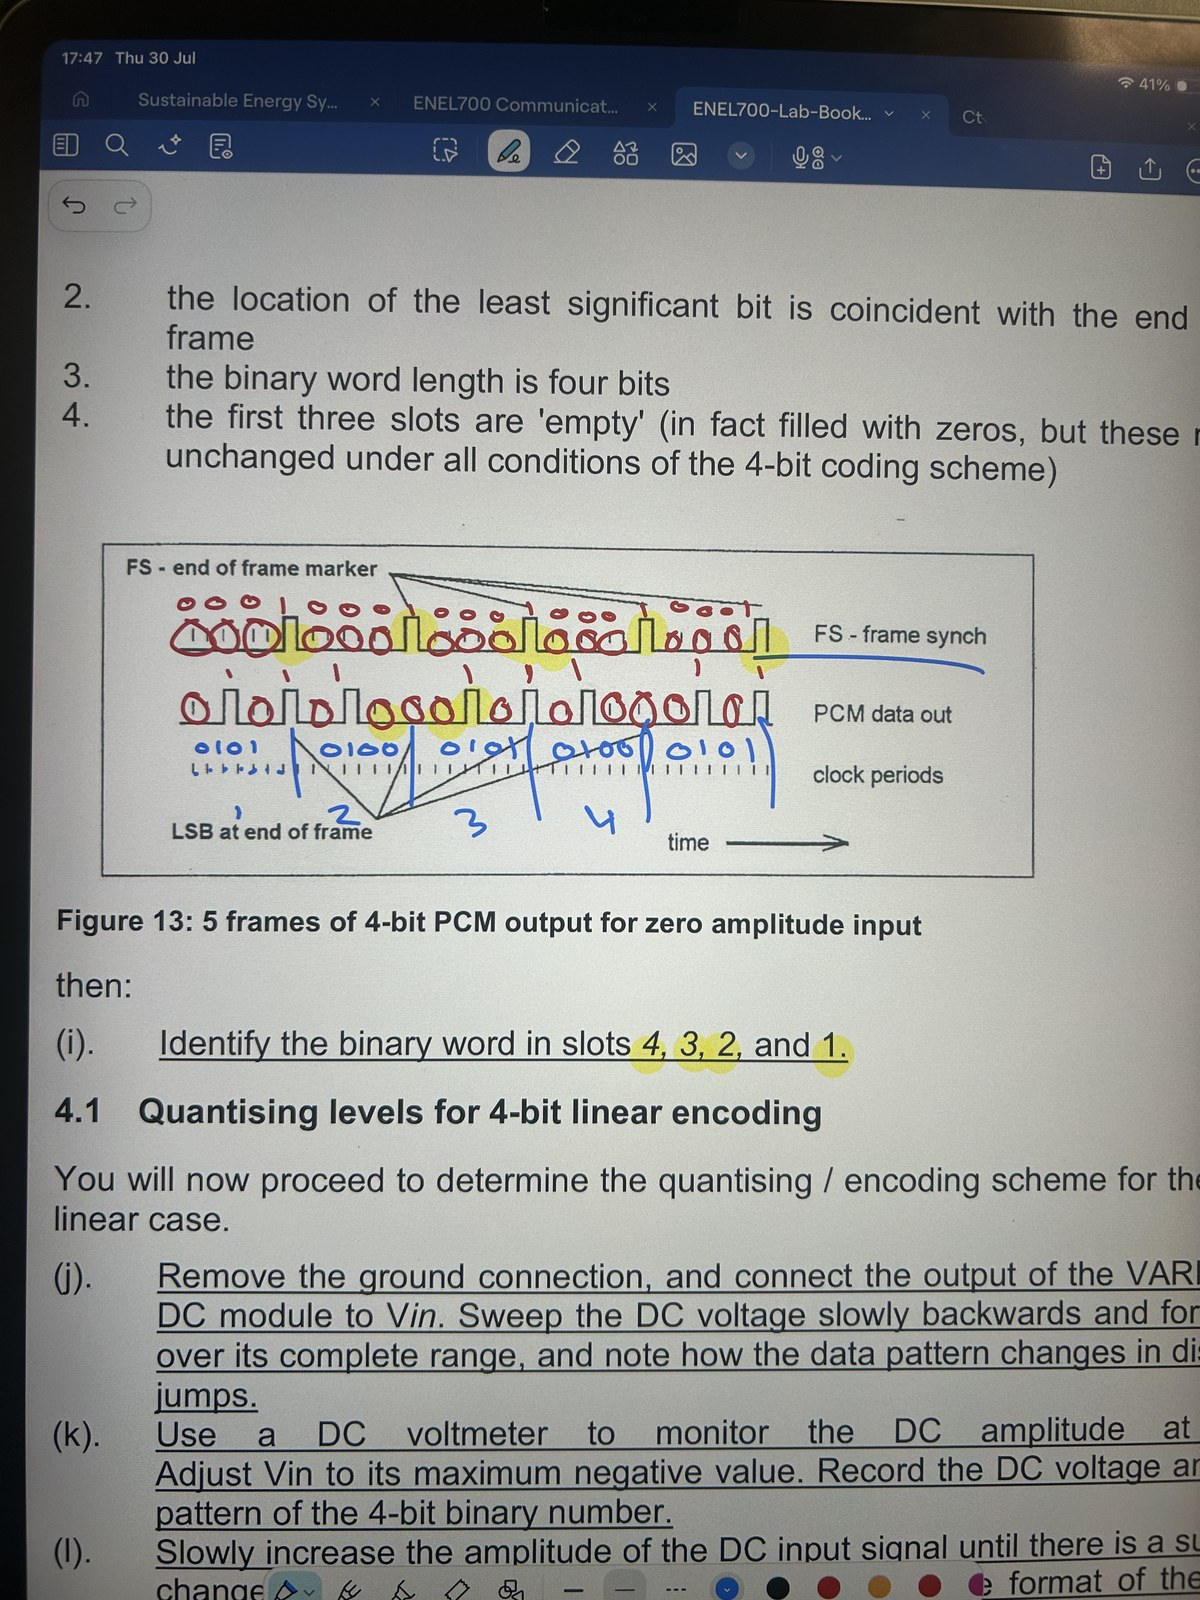
\includegraphics[width=0.55\textwidth]{lab4_decoding_note.jpg}
  \caption{Our in-class working note used to identify the four data-bit positions in each PCM frame.}
  \label{fig:lab4-note}
\end{figure}

\subsection{Question 4.1 raw linear data}

\begin{longtable}{r r c r}
\toprule
No. & $V_{in}$ (V) & Binary code & Decimal code \\
\midrule
\endhead
1 & $-2.635$ & 0000 & 0 \\
2 & $-2.239$ & 0001 & 1 \\
3 & $-1.911$ & 0010 & 2 \\
4 & $-1.595$ & 0011 & 3 \\
5 & $-1.277$ & 0100 & 4 \\
6 & $-0.960$ & 0101 & 5 \\
7 & $-0.308$ & 0110 & 6 \\
8 & $-0.270$ & 0111 & 7 \\
9 & $-0.020$ & 1000 & 8 \\
10 & $0.296$ & 1001 & 9 \\
11 & $0.645$ & 1010 & 10 \\
12 & $0.840$ & 1011 & 11 \\
13 & $1.314$ & 1100 & 12 \\
14 & $1.608$ & 1101 & 13 \\
15 & $2.062$ & 1110 & 14 \\
16 & $2.633$ & 1111 & 15 \\
\bottomrule
\end{longtable}

\begin{figure}[H]
  \centering
  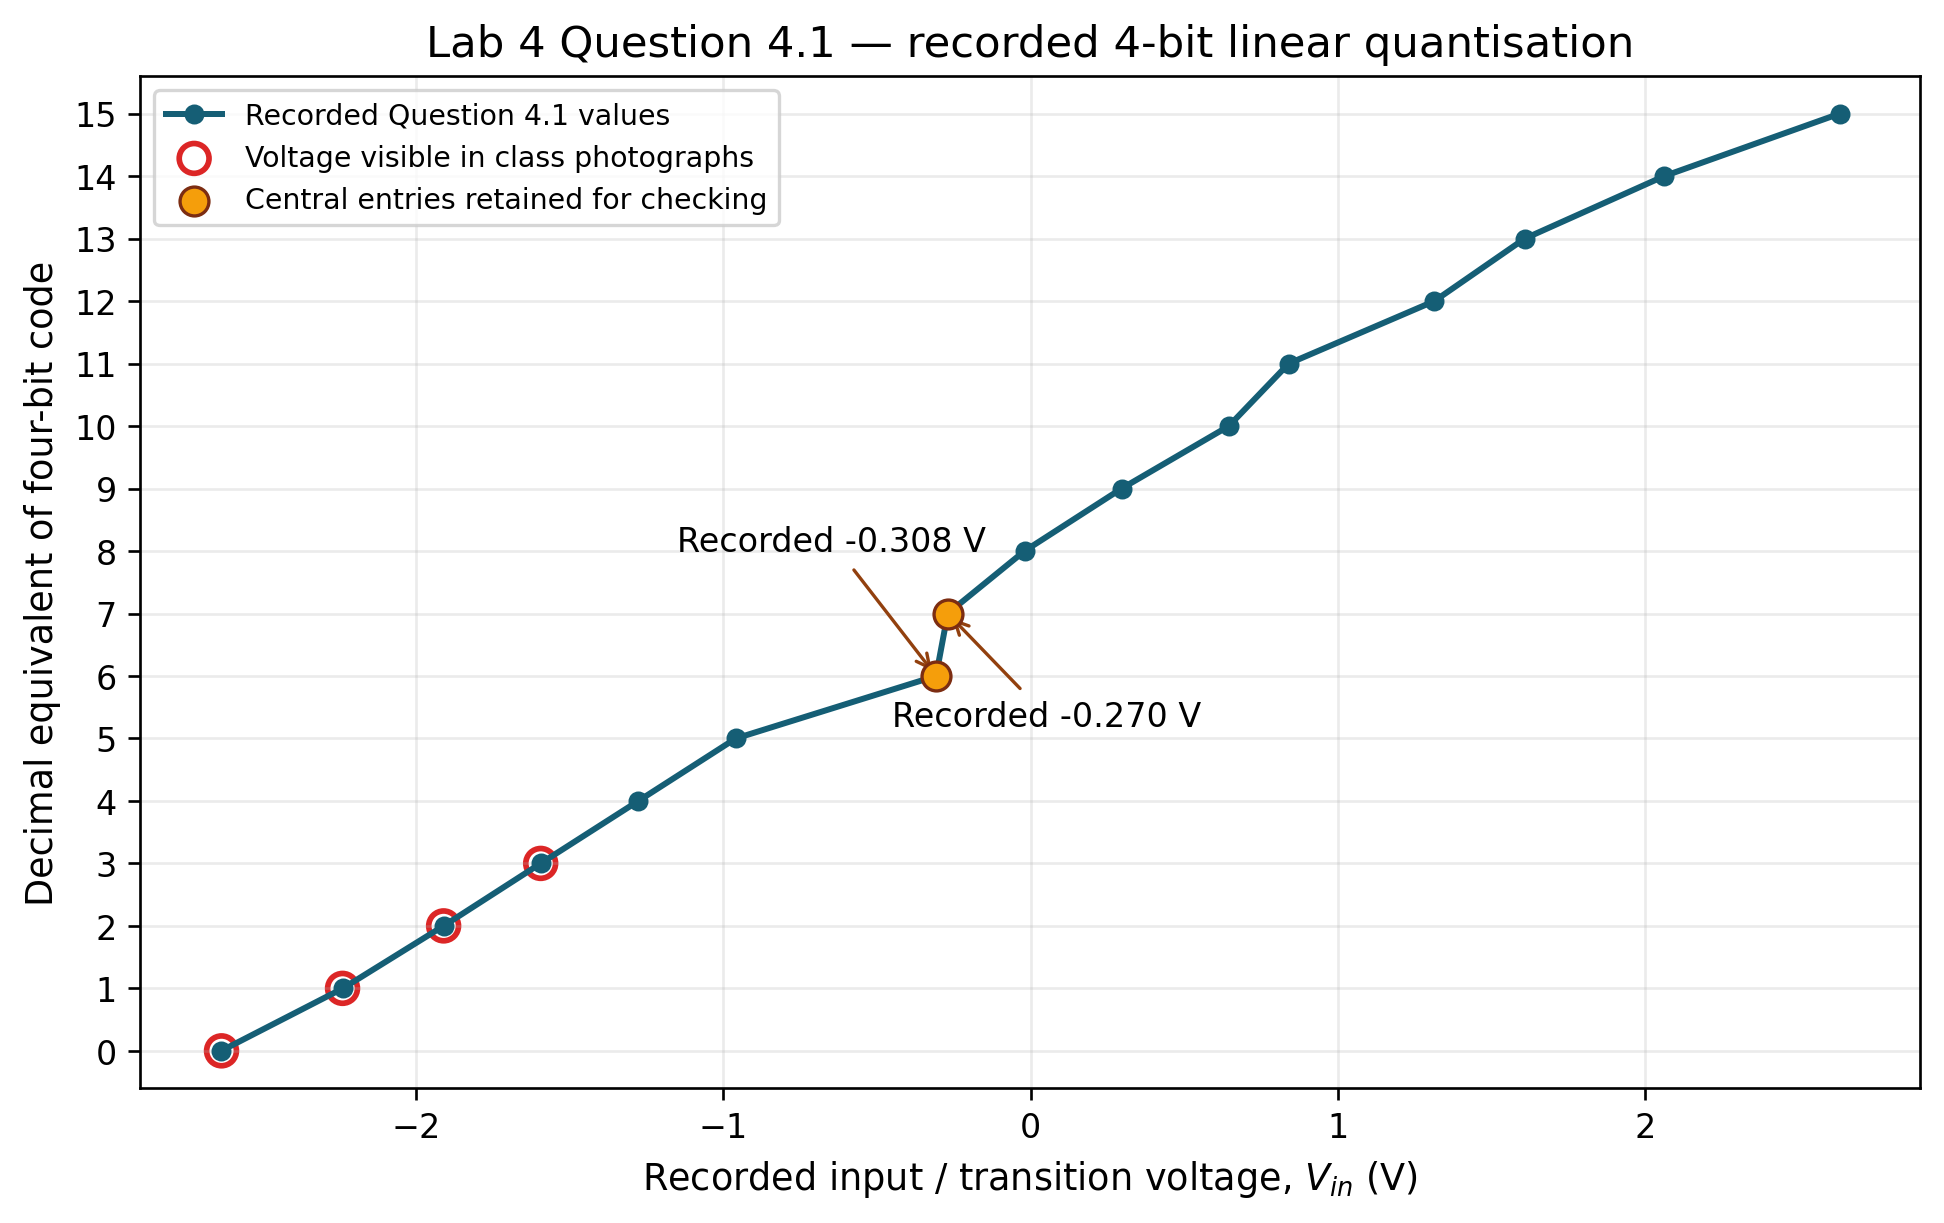
\includegraphics[width=0.96\textwidth]{lab4_q41_linear_raw.png}
  \caption{My graph of the Question 4.1 values exactly as recorded. The red rings mark values independently supported by class photographs. I retained the two questionable central entries and marked them in amber.}
  \label{fig:q41-linear}
\end{figure}

Across the full recorded range, the mean change is approximately $0.3512$ V per code step. The median adjacent spacing is approximately $0.318$ V. However, the recorded adjacent spacings range from $0.038$ V to $0.652$ V, largely because of the central entries. I therefore conclude that the result is broadly consistent with a linear 4-bit progression, but the typed table is not accurate enough to demonstrate uniform spacing quantitatively without checking the original hardcopy.

\begin{figure}[H]
\centering
\begin{subfigure}[t]{0.49\textwidth}
  \centering
  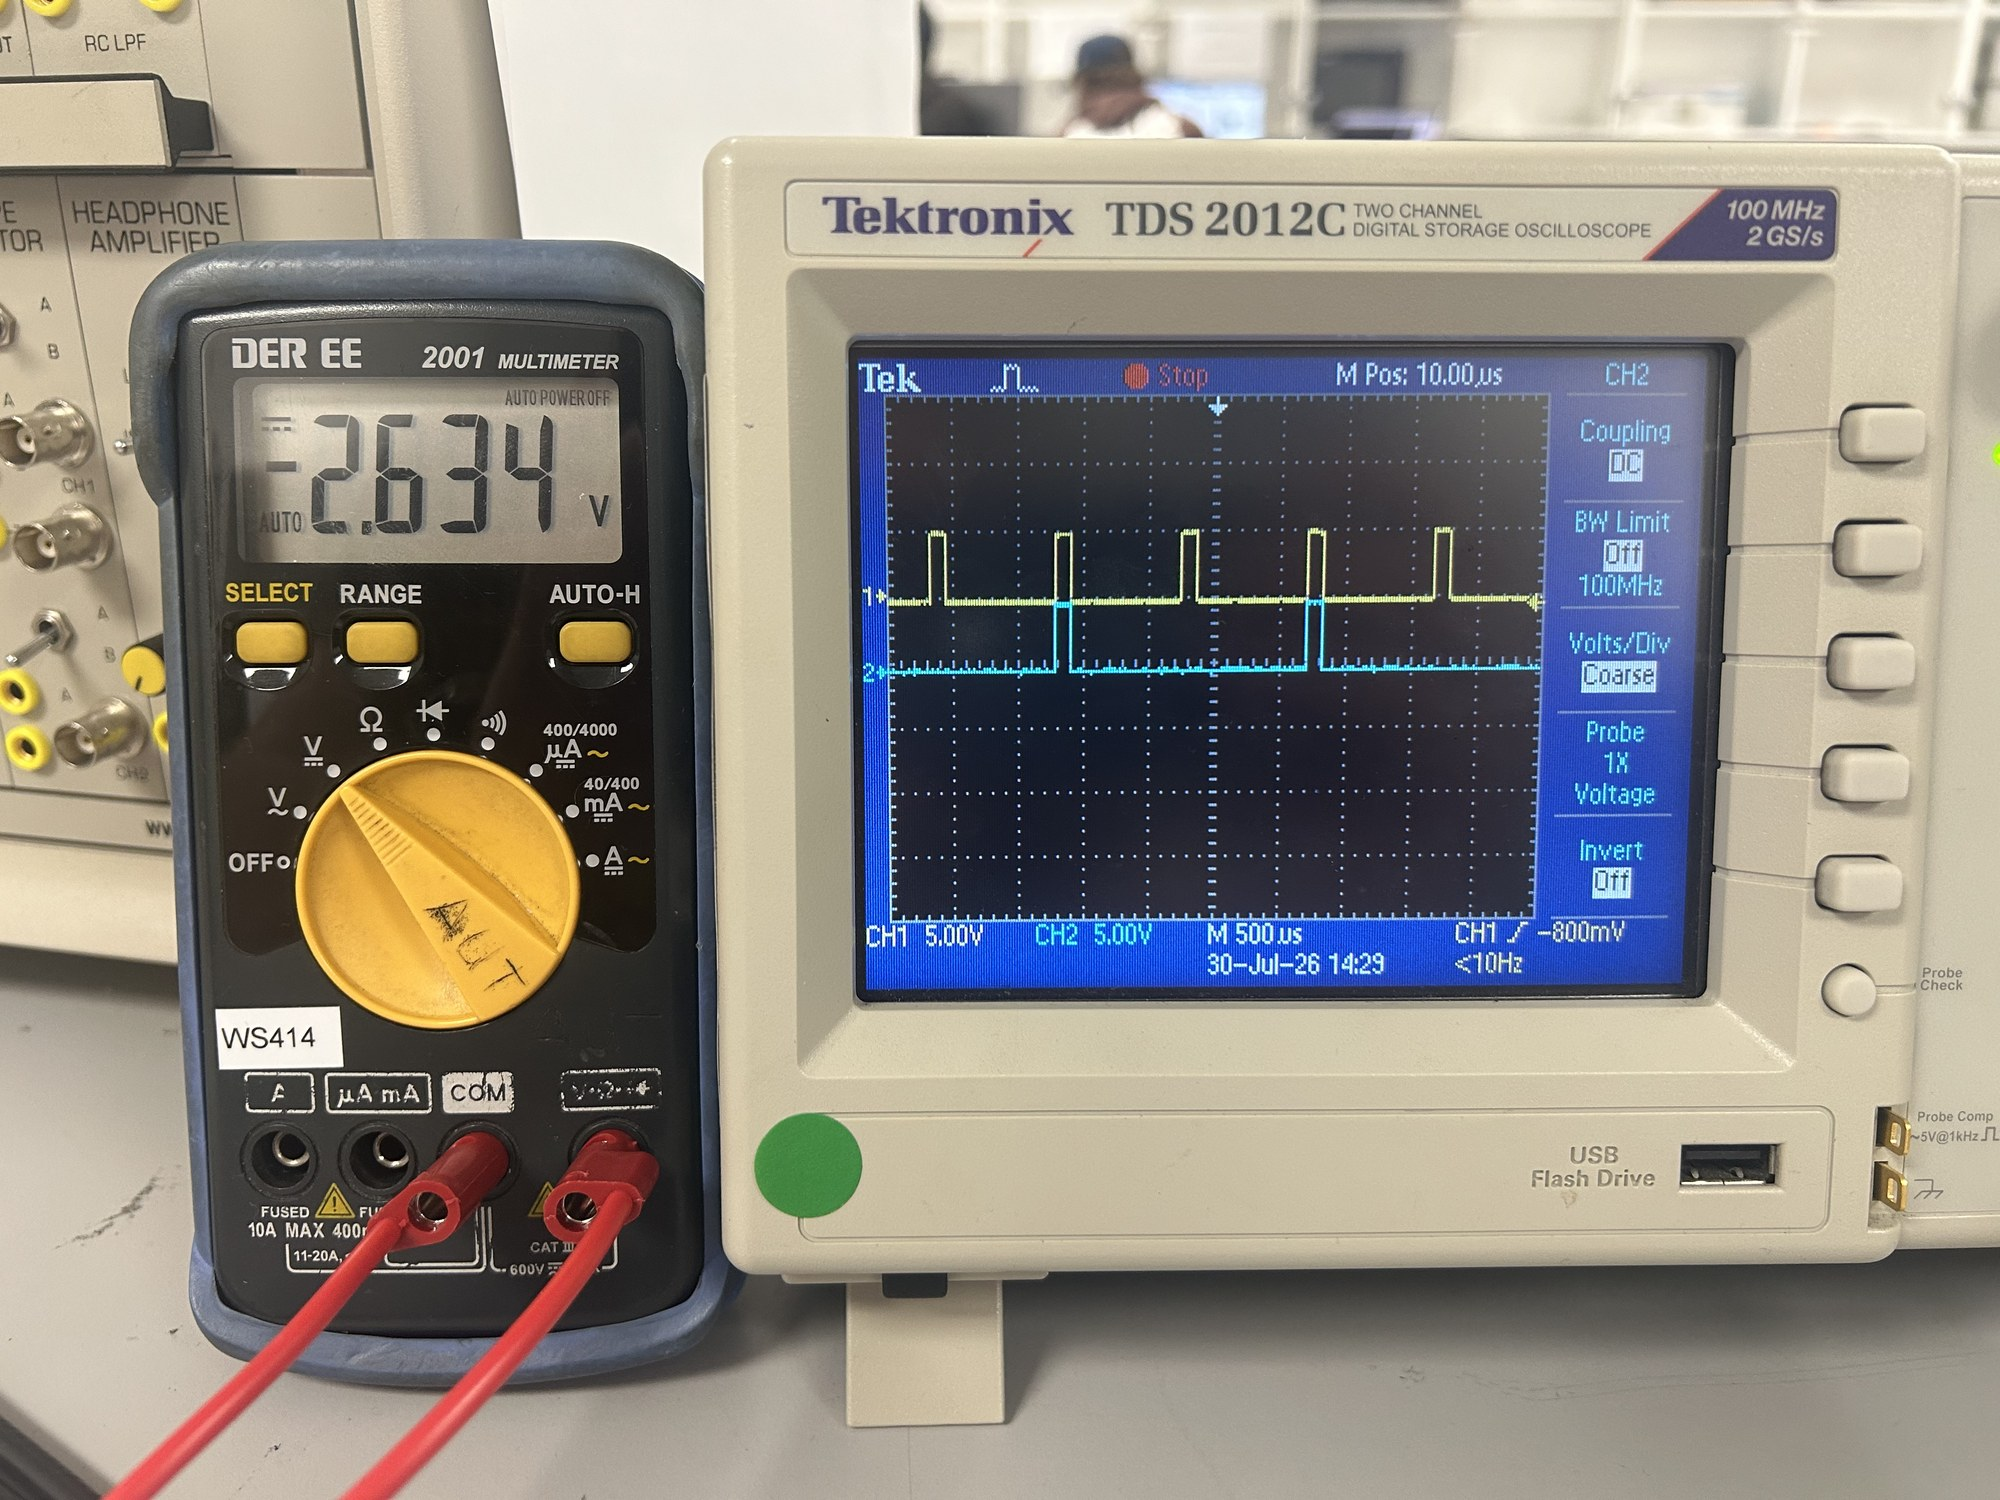
\includegraphics[width=\linewidth]{lab4_q41_minus2634.jpg}
  \caption{$-2.634$ V, code 0000.}
\end{subfigure}\hfill
\begin{subfigure}[t]{0.49\textwidth}
  \centering
  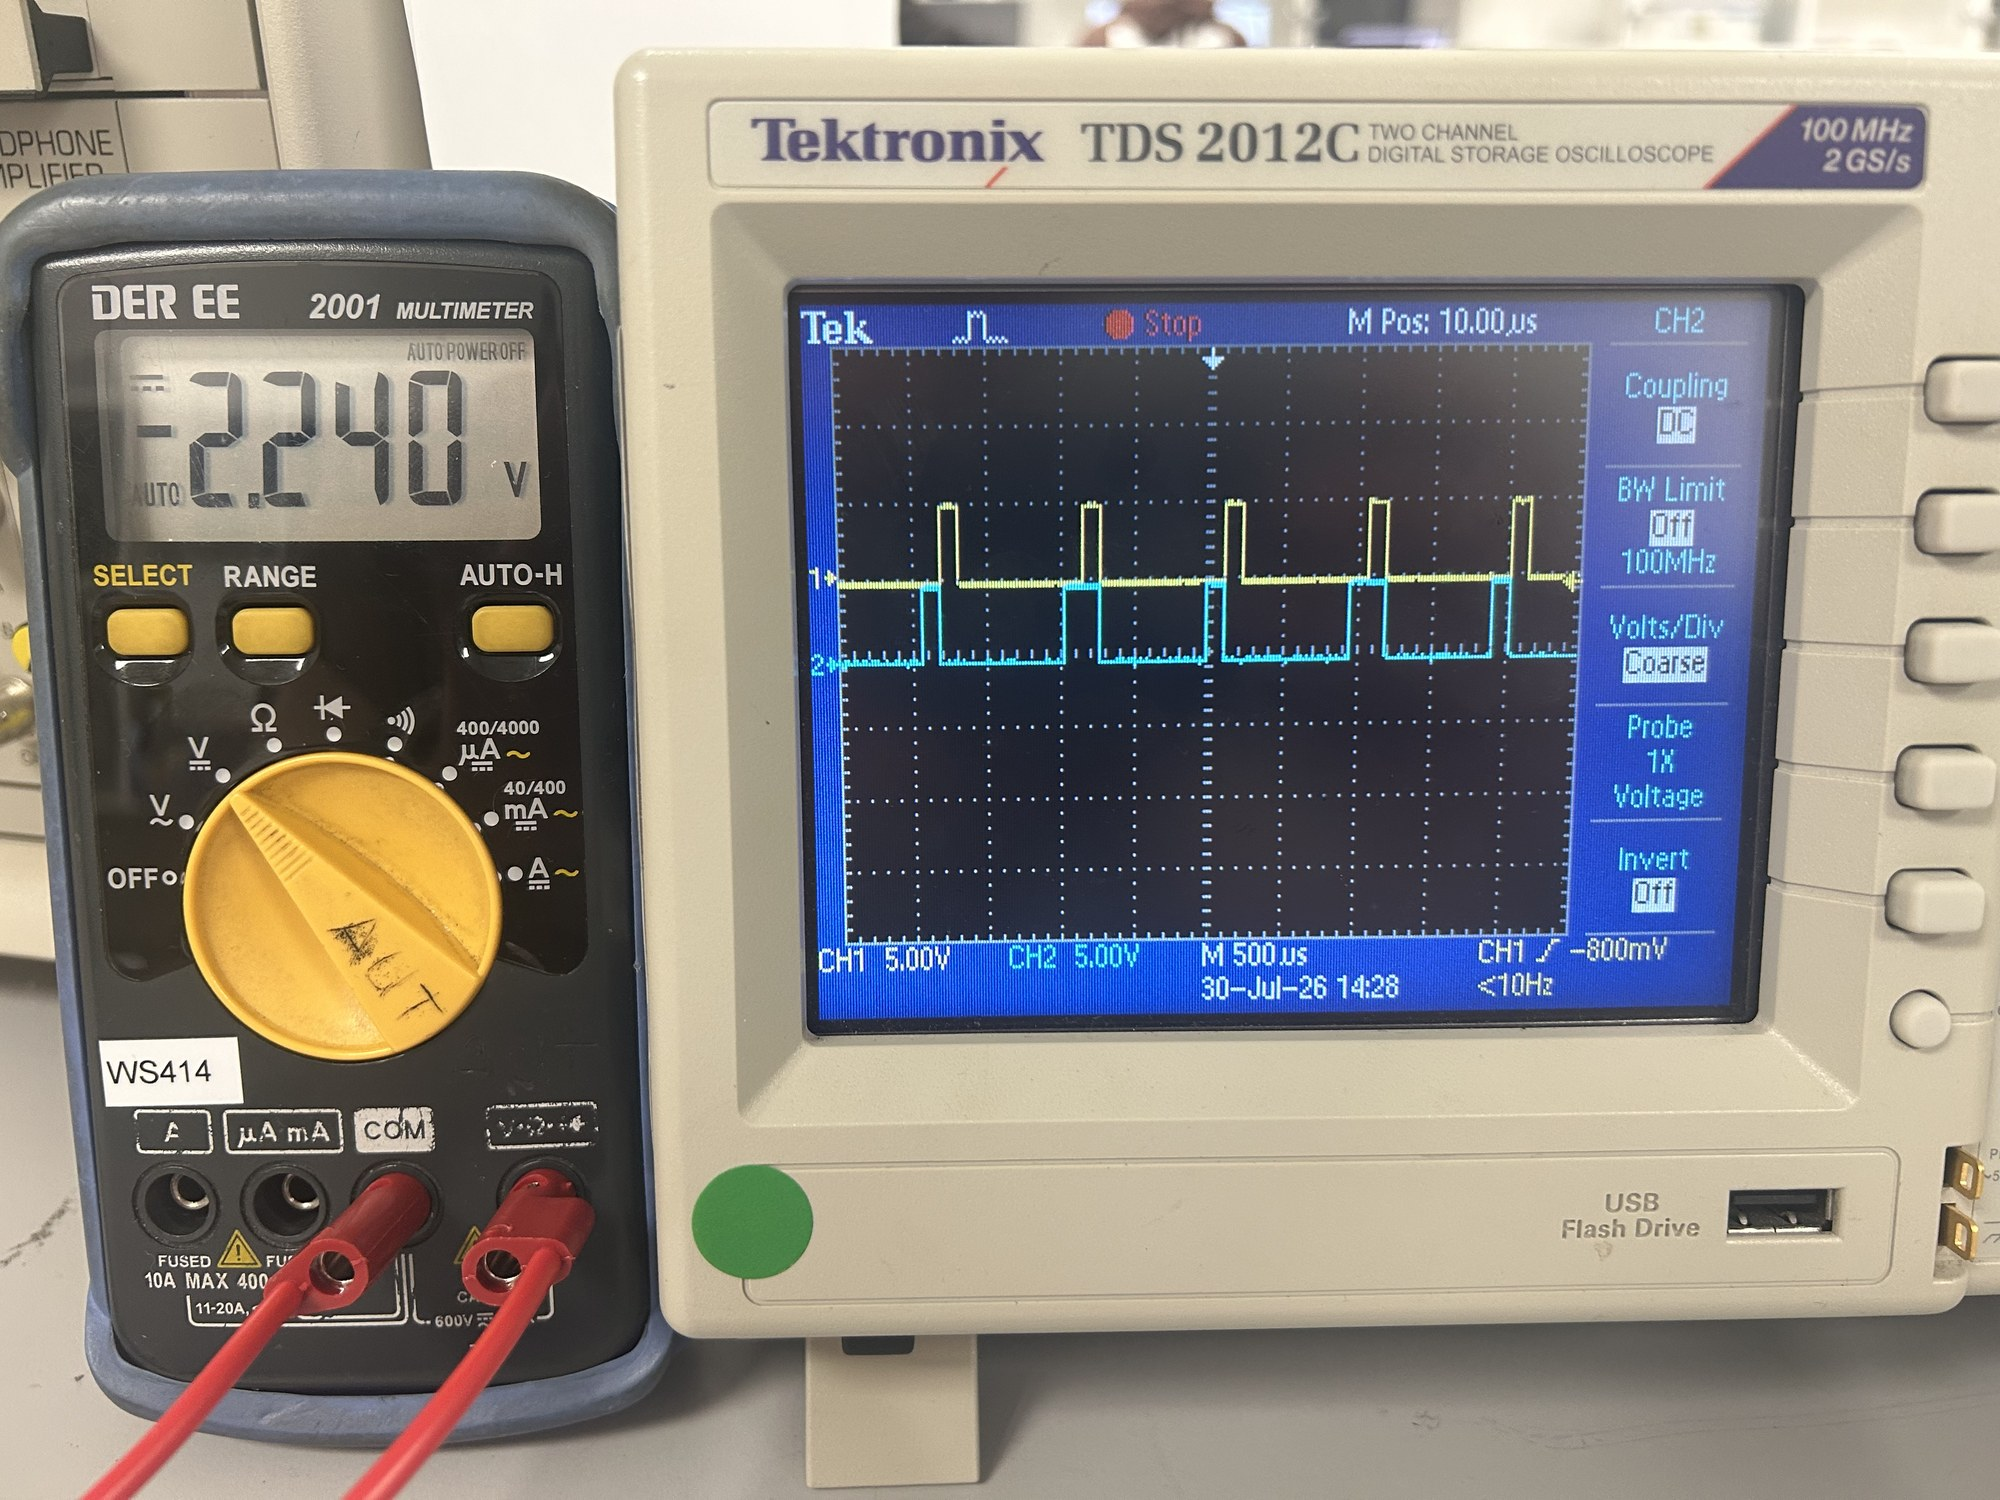
\includegraphics[width=\linewidth]{lab4_q41_minus2240.jpg}
  \caption{$-2.240$ V, code 0001.}
\end{subfigure}

\begin{subfigure}[t]{0.49\textwidth}
  \centering
  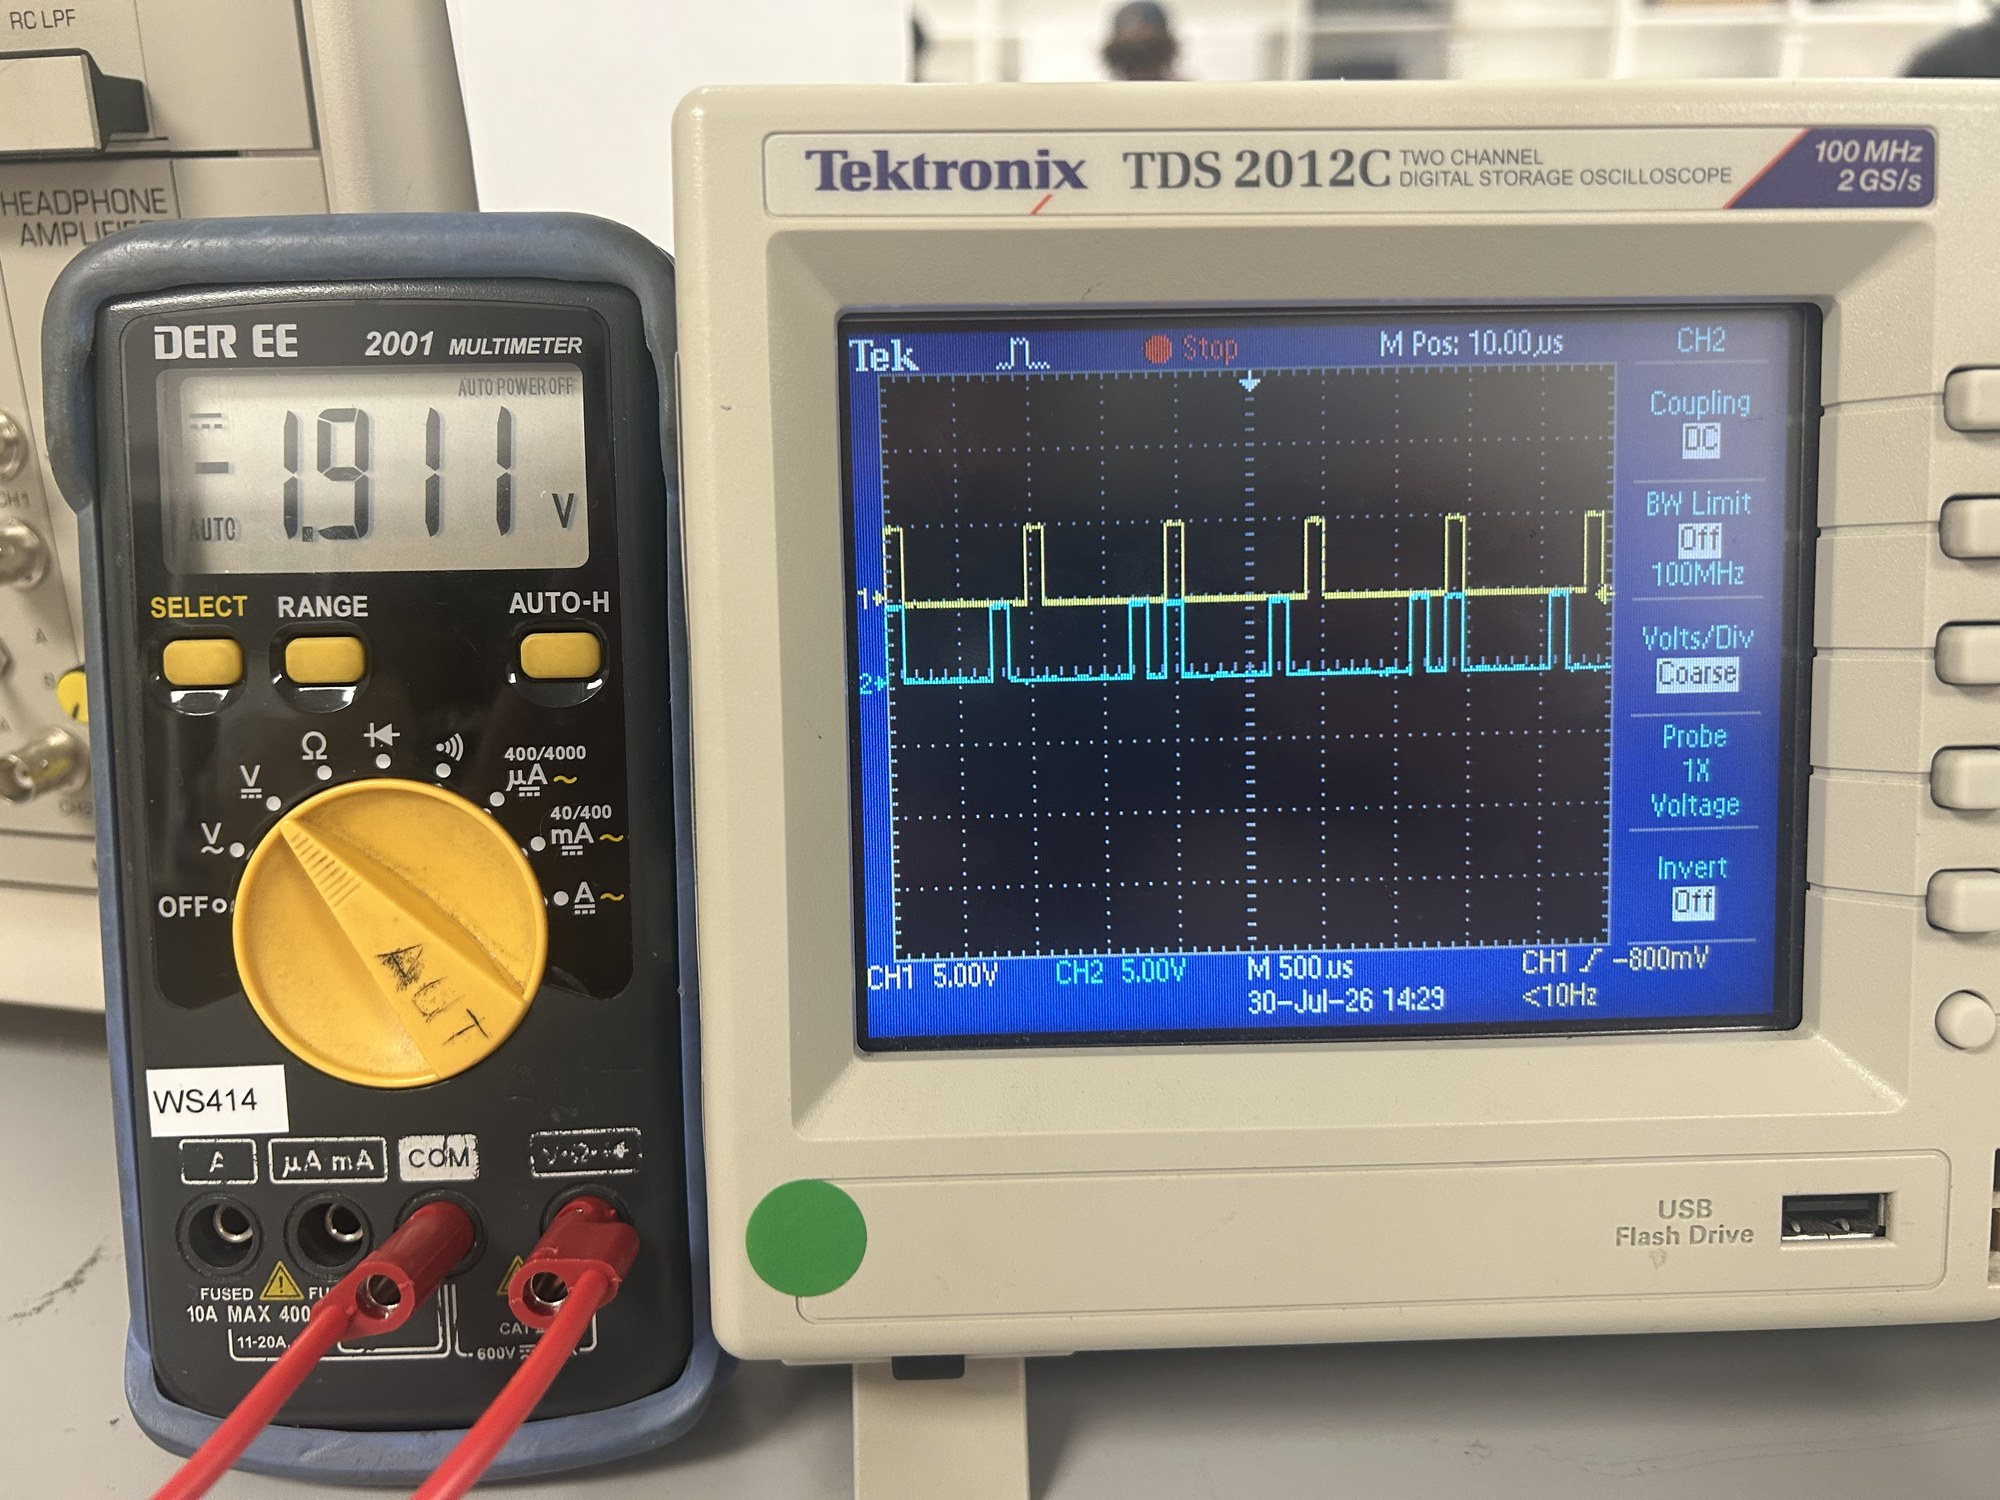
\includegraphics[width=\linewidth]{lab4_q41_minus1911.jpg}
  \caption{$-1.911$ V, code 0010.}
\end{subfigure}\hfill
\begin{subfigure}[t]{0.49\textwidth}
  \centering
  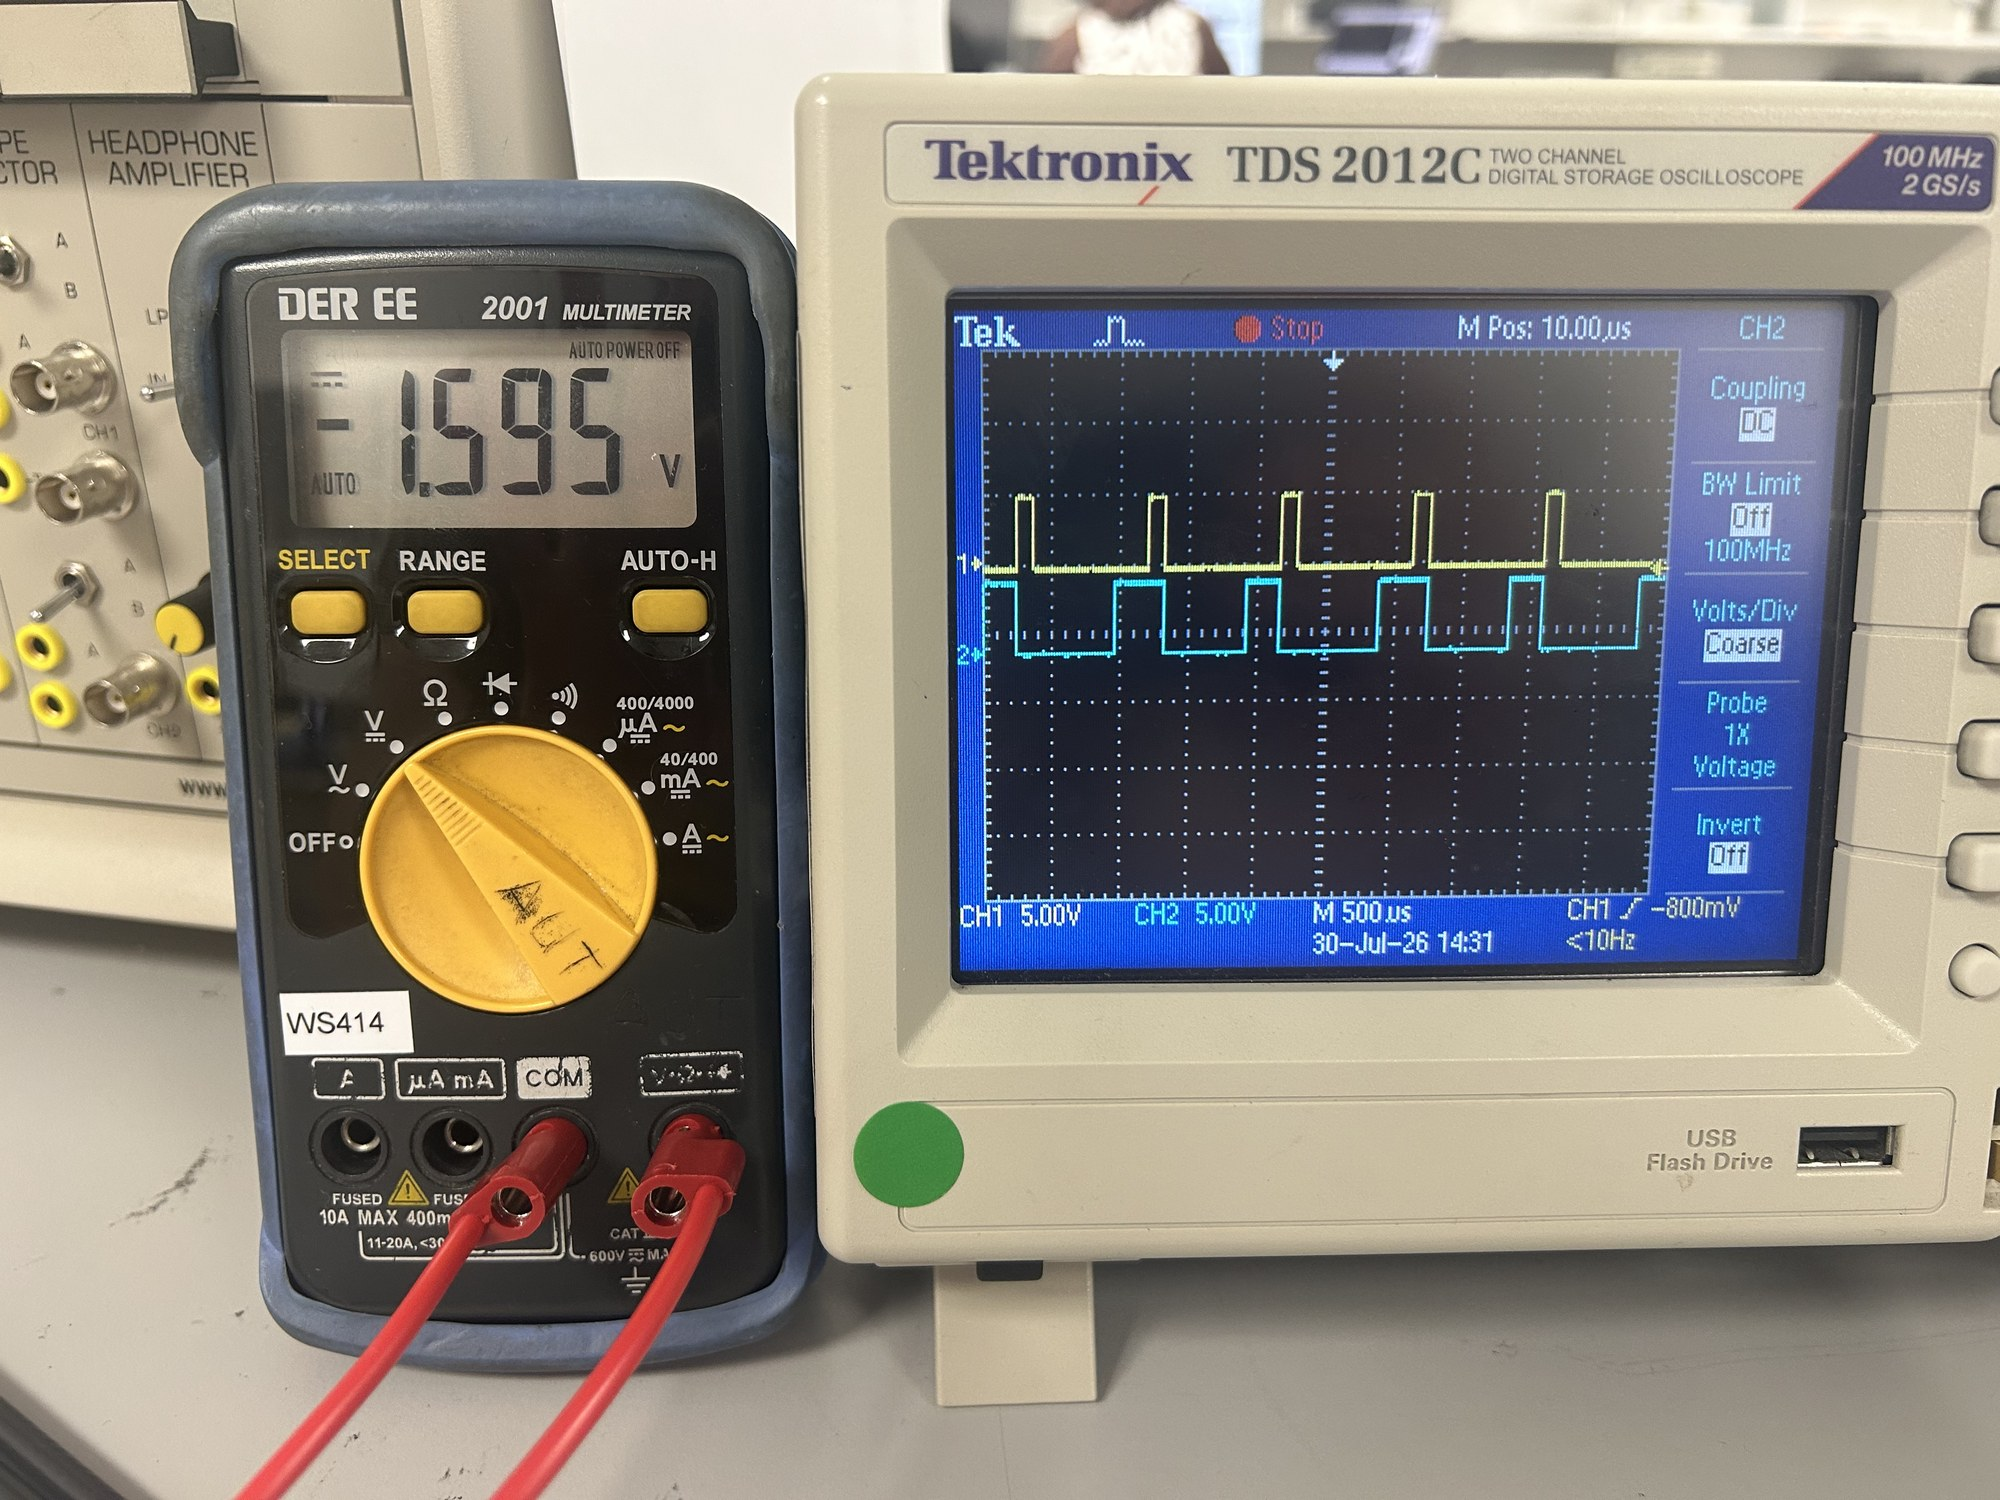
\includegraphics[width=\linewidth]{lab4_q41_minus1595.jpg}
  \caption{$-1.595$ V, code 0011.}
\end{subfigure}
\caption{Primary in-class photographic support for the first four Question 4.1 values. The meter signs and digits were checked directly at full resolution.}
\label{fig:q41-photos}
\end{figure}

\subsection{Question 4.2 partial companded data}

\begin{longtable}{r r c r}
\toprule
No. & $V_{in}$ (V) & Binary code & Decimal code \\
\midrule
\endhead
1 & $-2.632$ & 0000 & 0 \\
2 & $-1.100$ & 0001 & 1 \\
3 & $-0.522$ & 0010 & 2 \\
4 & $-0.291$ & 0011 & 3 \\
5 & $-0.154$ & 0100 & 4 \\
6 & $-0.003$ & 1001 & 9 \\
7 & $-0.072$ & 1011 & 11 \\
8 & $0.217$ & 1100 & 12 \\
9 & $0.308$ & 1101 & 13 \\
10 & $0.809$ & 1110 & 14 \\
11 & $1.272$ & 1111 & 15 \\
\bottomrule
\end{longtable}

\begin{figure}[H]
  \centering
  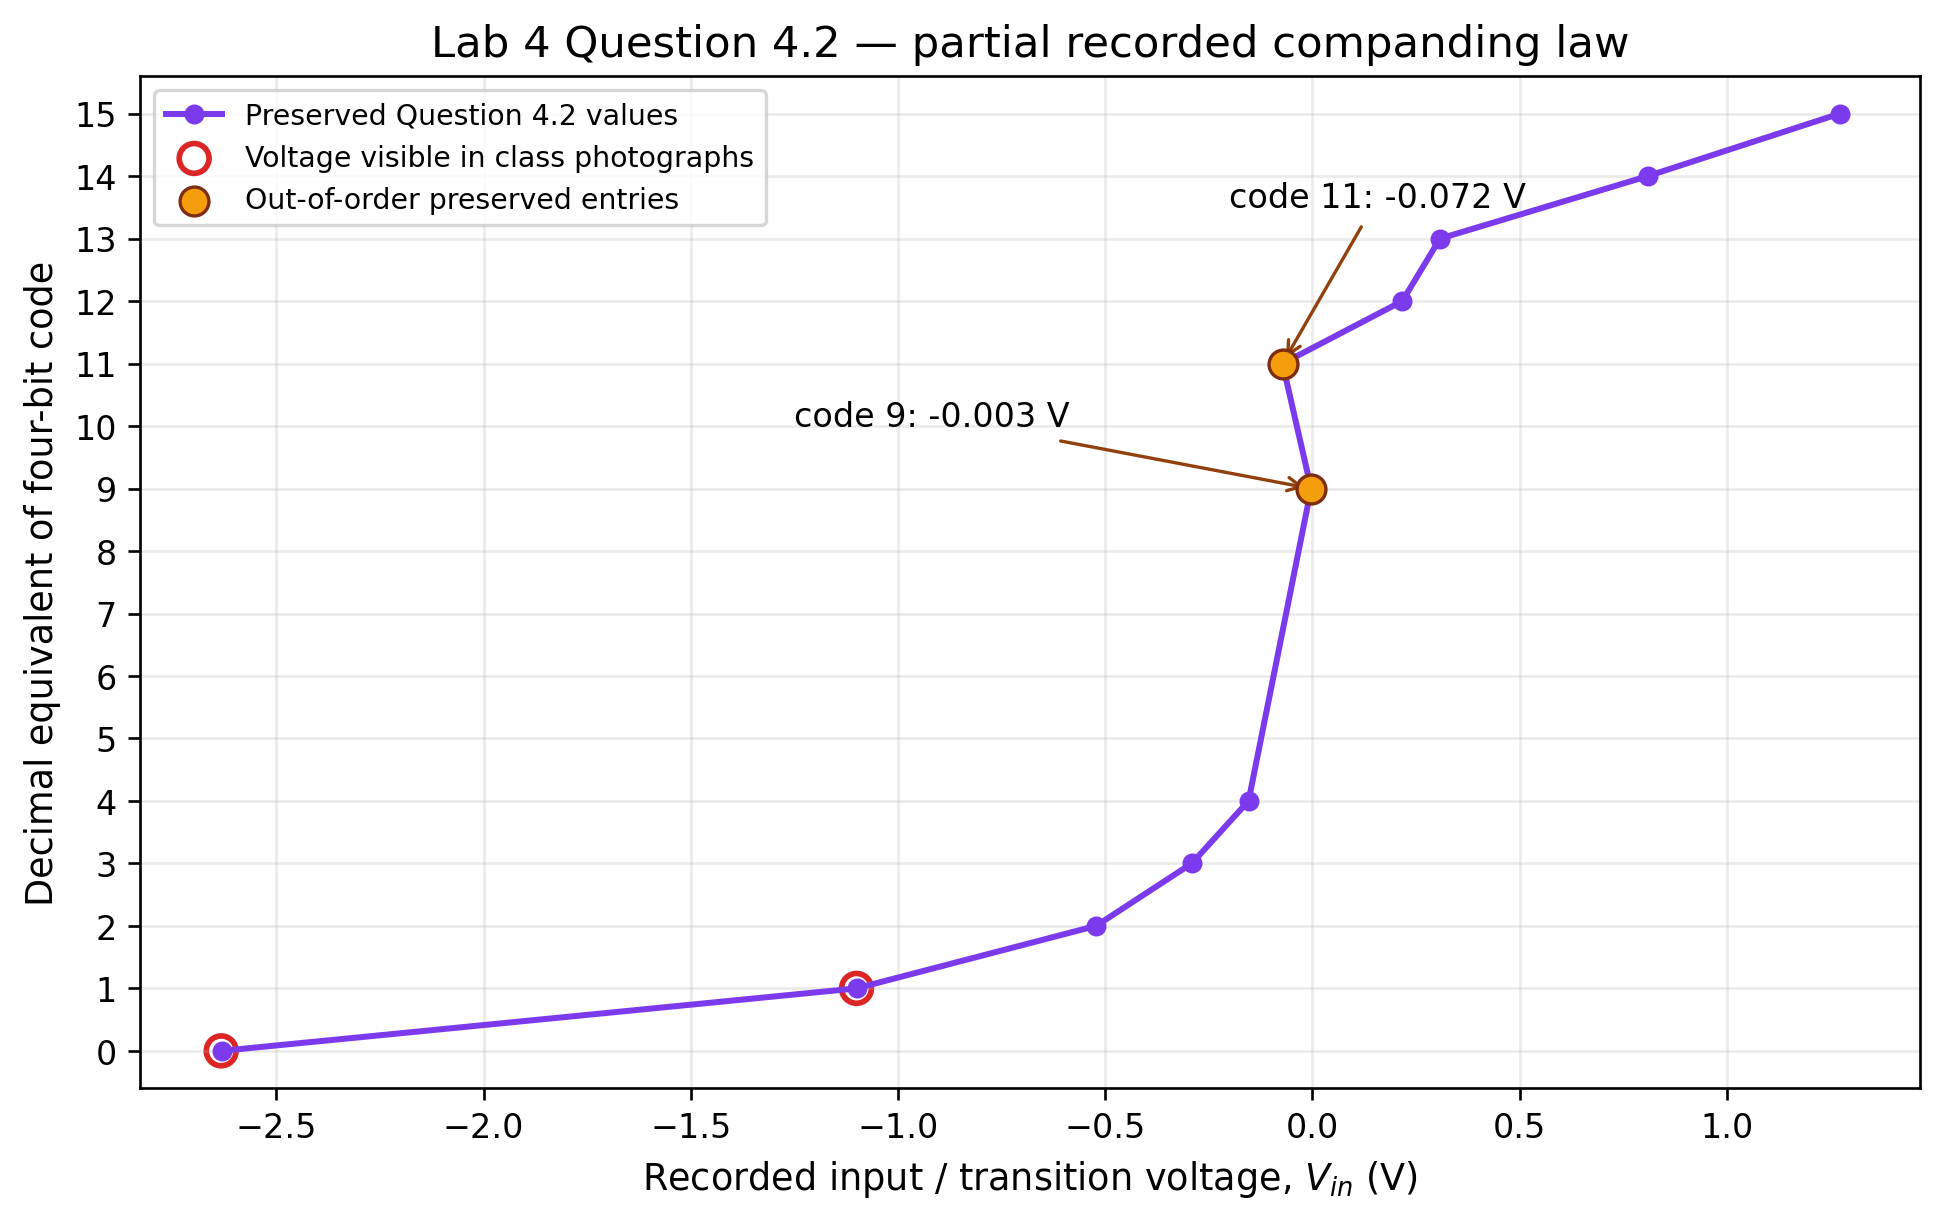
\includegraphics[width=0.96\textwidth]{lab4_q42_companding_partial.png}
  \caption{My graph of the partial Question 4.2 data. Missing codes create gaps, and the preserved code-9/code-11 pair is not monotonic. I show these limitations instead of interpolating invented measurements.}
  \label{fig:q42-compand}
\end{figure}

\begin{figure}[H]
\centering
\begin{subfigure}[t]{0.49\textwidth}
  \centering
  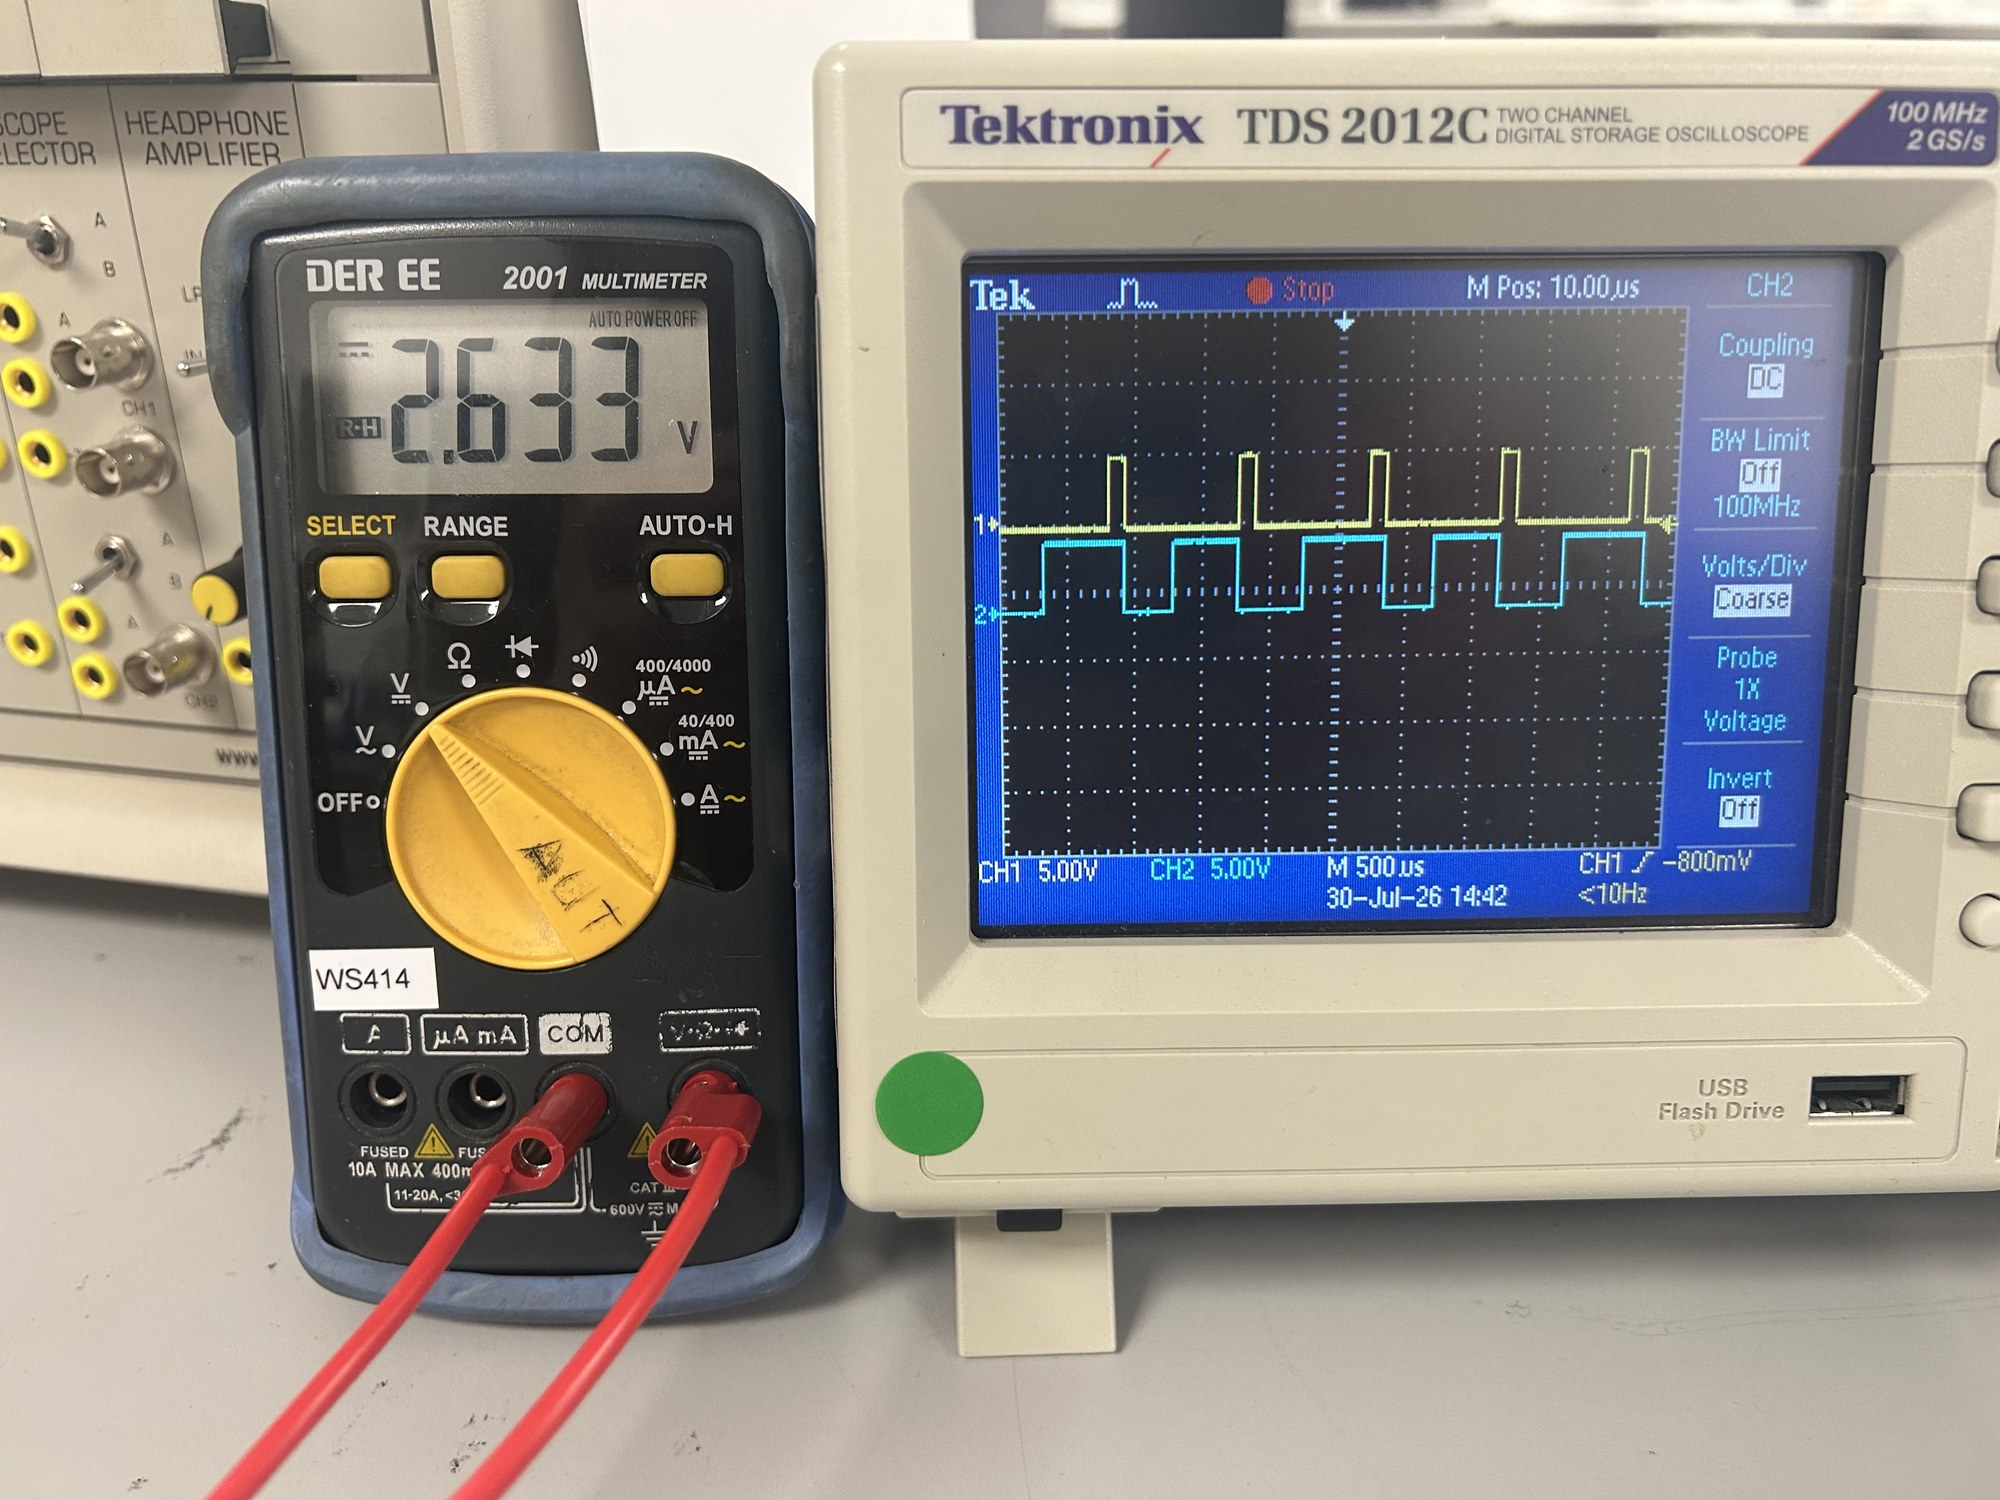
\includegraphics[width=\linewidth]{lab4_q42_minus2633.jpg}
  \caption{$-2.633$ V, matching code 0000.}
\end{subfigure}\hfill
\begin{subfigure}[t]{0.49\textwidth}
  \centering
  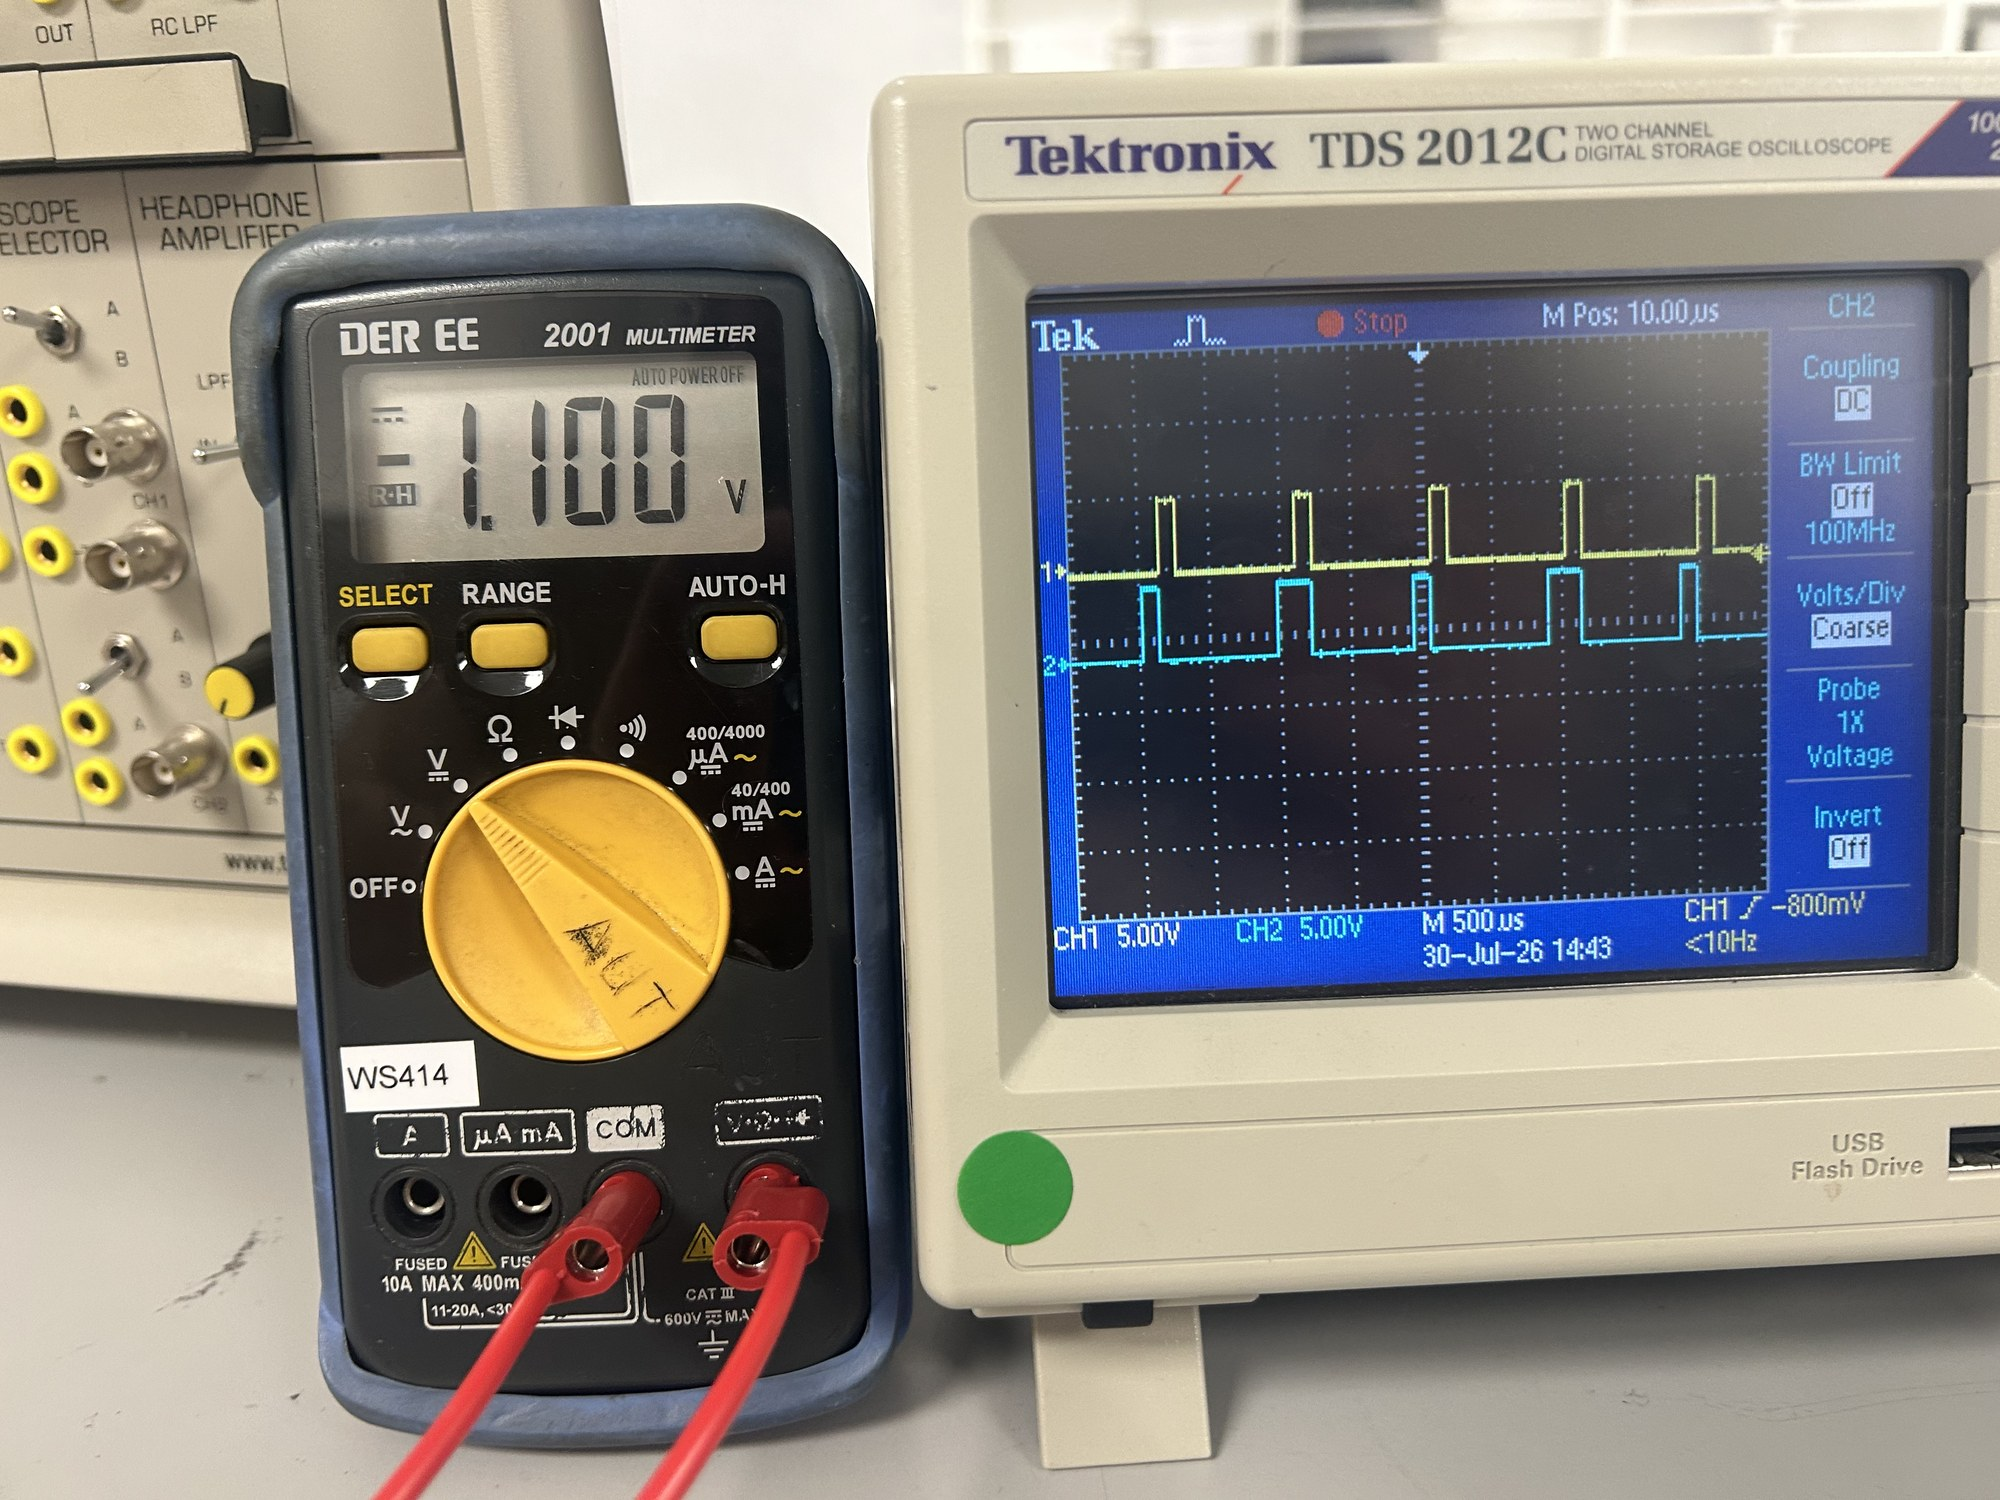
\includegraphics[width=\linewidth]{lab4_q42_minus1100.jpg}
  \caption{$-1.100$ V, matching code 0001.}
\end{subfigure}
\caption{Primary in-class photographic support for the first two Question 4.2 values.}
\label{fig:q42-photos}
\end{figure}

\begin{figure}[H]
  \centering
  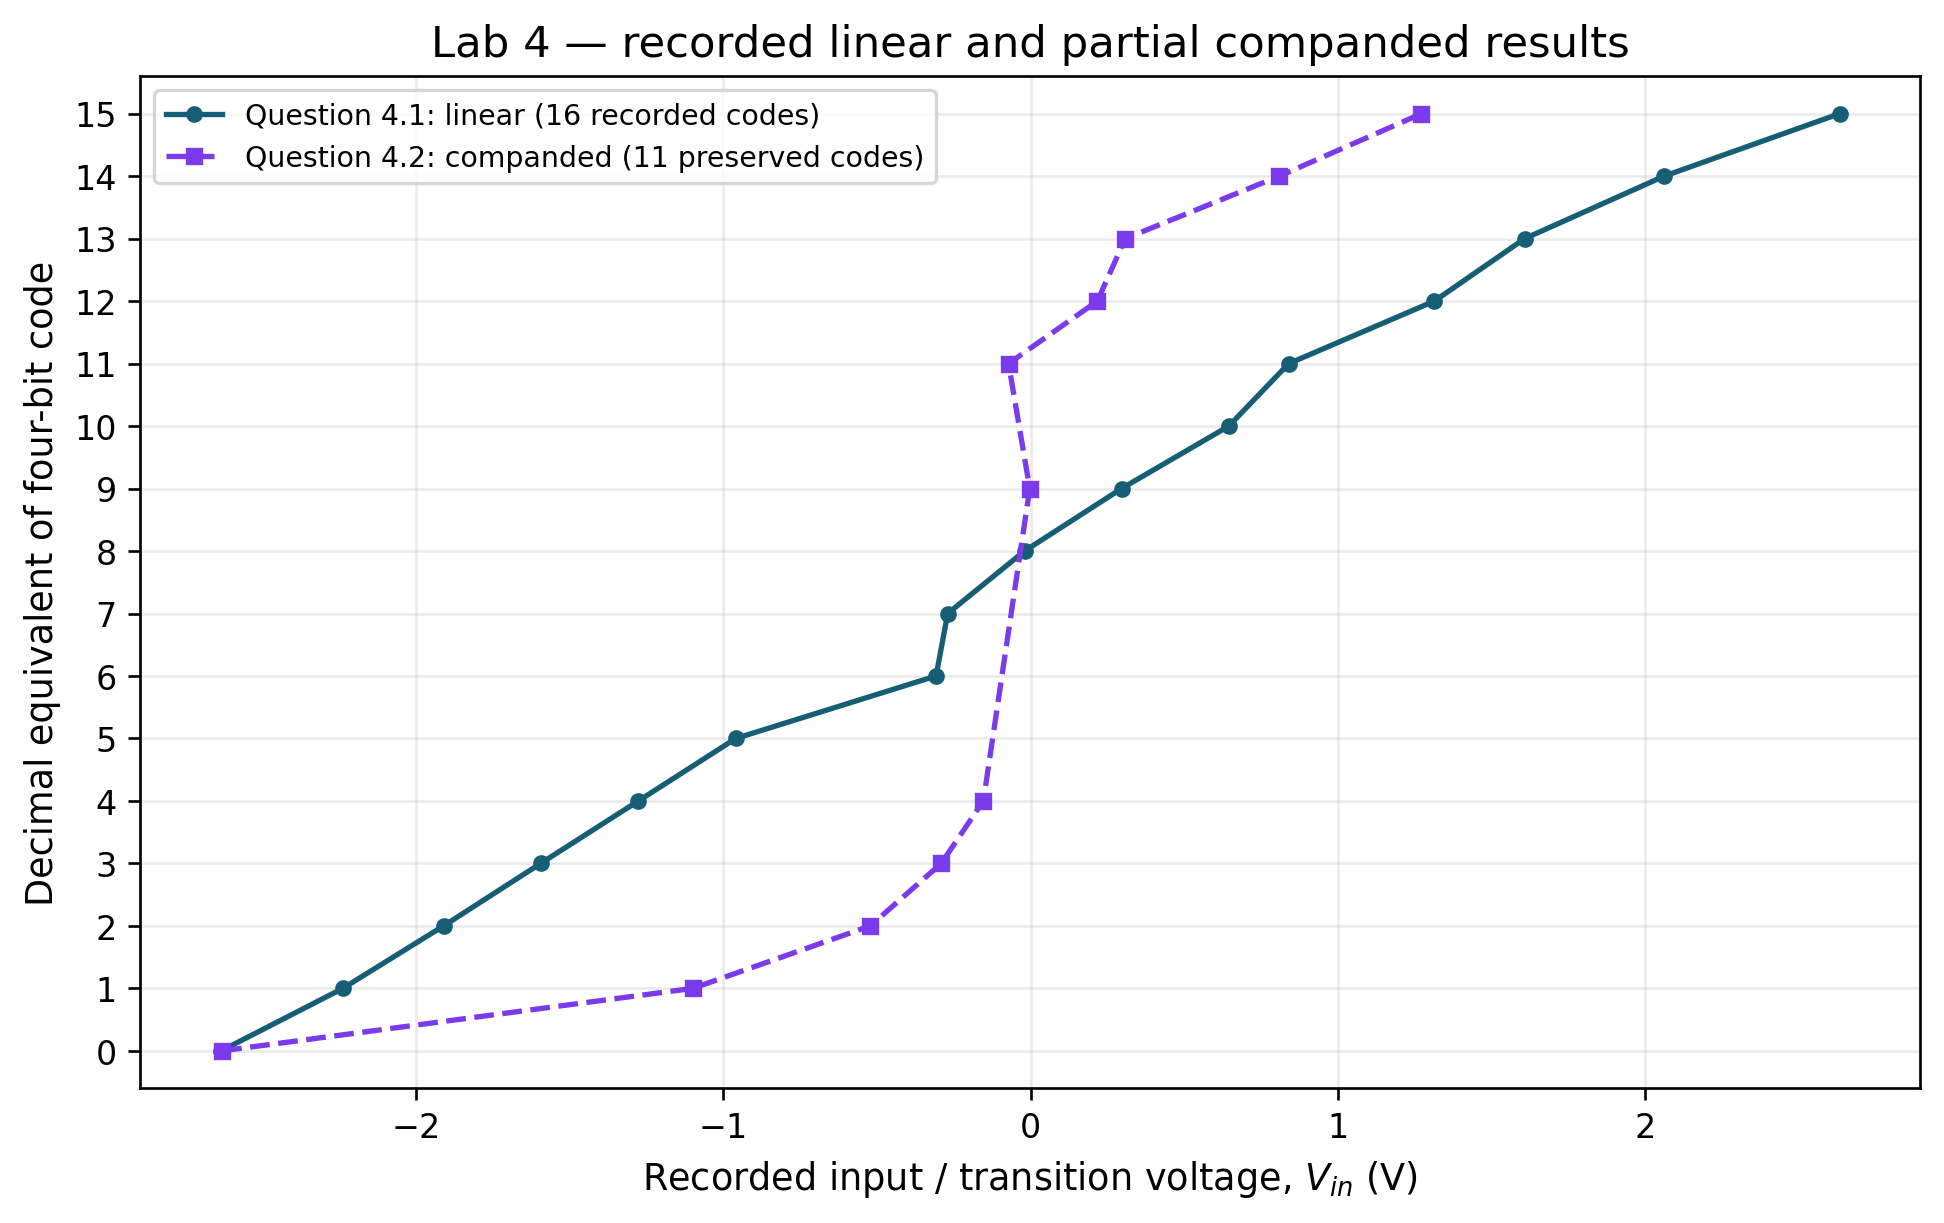
\includegraphics[width=0.96\textwidth]{lab4_linear_companded_comparison.png}
  \caption{Direct comparison of my complete raw linear sequence and the partial preserved companded sequence. This plot shows the expected non-uniform character qualitatively, but the incomplete and out-of-order companded record prevents a final quantitative companding-law fit.}
  \label{fig:comparison}
\end{figure}

\FloatBarrier
\section{Lab 4 manual questions answered}

\subsection{Question 1: sampling rate and input bandwidth}
\begin{answerbox}
The master clock was $f_{CLK}=8.333$ kHz and one PCM frame occupied eight clock periods. I calculated
\[
 f_s=\frac{8333}{8}=1041.625\ \text{samples/s}.
\]
This is the same for 4-bit and 7-bit coding because the TIMS frame remains eight slots long in both modes; the selected mode changes the number of data slots used, not the frame rate. By the Nyquist criterion, the theoretical maximum input bandwidth is
\[
 B_{max}=\frac{f_s}{2}=520.8125\ \text{Hz}.
\]
In practice, I would keep the message below this boundary and use suitable anti-alias filtering.
\end{answerbox}

\subsection{Question 2: 4-bit timing and quantisation}
\begin{answerbox}
\begin{enumerate}[label=(\alph*)]
\item Sampling rate: $1041.625$ samples/s.
\item Frame width: $8/8333=0.960038$ ms.
\item Data-bit width: $1/8333=120.005$ $\mu$s.
\item Four-bit data-word width: $4/8333=480.019$ $\mu$s.
\item Number of quantising levels: $2^4=16$.
\item The ideal 4-bit linear mode should have uniformly spaced levels. My raw graph is broadly increasing and covers all 16 codes, but the transcribed central values make the measured spacing non-uniform. I cannot honestly claim close uniformity until those entries are checked.
\end{enumerate}
\end{answerbox}

\subsection{Question 3: definition and composition of a frame}
\begin{answerbox}
I define a frame as the eight-clock-slot interval used to carry the encoded value of one analogue sample together with synchronisation information. In 4-bit mode, slots 7--5 remain zero, slots 4--1 carry the four-bit data word, and slot 0 carries the encoder's alternating embedded frame-synchronisation bit.

\begin{center}
\begin{tabular}{c|c|c|c|c|c|c|c|c}
\toprule
Slot & 7 & 6 & 5 & 4 & 3 & 2 & 1 & 0 \\
\midrule
Content & 0 & 0 & 0 & $D_3$ & $D_2$ & $D_1$ & $D_0$ & FS \\
\bottomrule
\end{tabular}
\end{center}
The FS bit alternates 1, 0, 1, 0 across successive frames. At 8.333 kHz, equal-valued embedded pulses recur every two frames, approximately $1.920$ ms apart.
\end{answerbox}

\subsection{Question 4: transmitting frames more slowly}
\begin{answerbox}
I could store completed frames in a buffer or memory, then transmit the stored bits using a slower serial clock and reconstruct their original timing at the receiver using a buffer, recovered clock and frame synchronisation. This introduces delay and requires enough storage. A continuously operating source cannot be sent forever at an average information rate below the rate at which bits are produced unless I also reduce, compress or discard information. Slower delayed transmission is useful for recorded data, burst transmission, time-division sharing, or a channel whose instantaneous rate is low but where delay is acceptable.
\end{answerbox}

\subsection{Question 5: stable and unstable oscilloscope displays}
\begin{answerbox}
A DC message is constant, so every sample is assigned the same quantisation code. Triggering on frame synchronisation overlays identical PCM frames and gives a stable display. With a sinusoidal message, the sample amplitude changes from frame to frame, so the encoder produces different code words. When those frames are repeatedly overlaid, the PCM data appears unstable or as many superimposed patterns unless I capture a single frame or synchronise over the complete repeating message sequence.
\end{answerbox}

\subsection{Question 6: quantisation diagram and experimental method}
\begin{answerbox}
Figure~\ref{fig:q41-linear} is my measured quantisation diagram. I started near the maximum negative input, read the four data bits in slots 4--1, converted each binary word to decimal, and slowly increased the Variable DC input. Each time the PCM word changed, Nahil and I recorded the meter voltage and the new code. We continued until the sequence reached 1111. The photograph series in Figure~\ref{fig:q41-photos} directly supports the first four measured code regions.
\end{answerbox}

\subsection{Question 7: reconstruction-filter amplitude characteristic}
\begin{answerbox}
I would require a low-pass filter with a substantially flat amplitude response across the wanted message band and strong attenuation at the sampling images above that band. If I am using the output to measure second- and third-order message harmonics, the passband must extend far enough to retain those harmonics; otherwise the filter would hide distortion and give a falsely optimistic result. Passband ripple should be small enough that it does not materially change the measured message amplitudes.
\end{answerbox}

\subsection{Question 8: reconstruction-filter specification}
\begin{answerbox}
I would start with the maximum wanted message frequency, the $1041.625$ samples/s sampling rate, and the location of the first spectral image. I would then specify: passband edge; acceptable passband ripple; stopband edge and attenuation; transition width; allowable phase or group-delay distortion; load and signal levels; and whether the second and third message harmonics must remain measurable. The final cutoff must pass the wanted content while rejecting the high-frequency sample-and-hold components as much as the available transition band allows.
\end{answerbox}

\subsection{Question 9: reducing sampling and quantisation distortion}
\begin{answerbox}
For sampling distortion from a sample-and-hold system, I can raise the sampling rate relative to the message bandwidth, use appropriate anti-alias and reconstruction filters, and compensate sample-and-hold aperture droop where necessary. For quantisation distortion, I can increase the number of bits and levels, scale the signal so it uses the available input range without clipping, or use a suitable non-uniform quantiser/compander for signals such as speech.
\end{answerbox}

\subsection{Question 10: cost of increasing the number of levels}
\begin{answerbox}
More quantisation levels require more bits per sample. The price is greater converter and decoder complexity, a higher serial bit rate or more occupied frame slots, more storage, wider channel bandwidth when the sample rate is unchanged, and potentially greater power and clocking demands. In this TIMS experiment, the cost was visible as extra data-bit positions: 7-bit mode uses seven data slots instead of four. Because the frame was fixed at eight clock periods, the sample rate itself remained unchanged, but the resolution and number of occupied data slots increased.
\end{answerbox}

\section{Lab 5 manual questions answered}

\subsection{Question 1: MATLAB spectrum function}
\begin{answerbox}
I completed the supplied \texttt{sigspec} structure by forcing row inputs into columns, applying a Hamming window, using a zero-padded FFT, centring the spectrum with \texttt{fftshift}, and plotting either linear magnitude or the manual's $10\log_{10}$ magnitude. The function I used for the completed written answer is listed below. The optional outputs let me verify the peak locations numerically; they do not change the required plotting behaviour.
\end{answerbox}

\begin{lstlisting}[style=matlab,caption={My completed Lab 5 \texttt{sigspec.m} function.}]
function [f, siginspec] = sigspec(sigin, flag)
%SIGSPEC Display a signal spectrum using the ENEL700 Lab 5 method.
% Optional outputs are retained only for numerical verification.
if(nargin==0)
    disp('USAGE: sigspec(sigin,flag)');
    disp('   The input signals should be in the columns of sigin.');
    disp('   flag=0 produces a linear magnitude plot (default)');
    disp('   flag=1 produces a log magnitude plot (dB)');
    f = [];
    siginspec = [];
    return;
end
if(nargin==1)
    flag = 0;
end
[len,numsigs]=size(sigin);
if(len<numsigs)
    sigin = sigin.';
    tmp = len;
    len = numsigs;
    numsigs = tmp;
end
fftsize = 2^(ceil(log2(len))+2);
f=[0:fftsize-1].'/fftsize - 0.5;
sigin = repmat(hamming(len),1,numsigs).*sigin;
siginspec = abs(fftshift(fft(sigin,fftsize),1));
if(flag)
    plot(f,10*log10(siginspec));
    ylabel('Magnitude (dB)');
else
    plot(f,siginspec);
    ylabel('Linear magnitude');
end
xlabel('Normalized Frequency');
end
\end{lstlisting}

\subsection{Question 2: explanation of the three spectra and scaling}
\begin{answerbox}
In the first plot, the modulating signal is a baseband signal, so most of its spectral energy is centred near normalized frequency zero. In the second plot, the sinusoidal carrier gives narrow symmetric components at approximately $-0.3$ and $+0.3$. In the third plot, multiplying the message by the carrier shifts copies of the message spectrum from baseband to regions around $-0.3$ and $+0.3$. Because this is suppressed-carrier modulation, I do not expect a separate dominant unmodulated carrier line in the output.

For a unit cosine carrier,
\[
\cos(2\pi f_c n)=\tfrac{1}{2}e^{j2\pi f_c n}+\tfrac{1}{2}e^{-j2\pi f_c n},
\]
so each shifted copy has one-half of the original message-spectrum magnitude. My later numerical check measured a ratio of $0.498366$, close to the expected $0.5$. Under the manual's $10\log_{10}$ convention, this was $-3.0245$ dB, close to the expected $-3.0103$ dB. Figure~\ref{fig:lab5-class-spectra} remains the primary in-class plot; Figure~\ref{fig:lab5-scaling} is a later calculation used to verify the expected scaling.
\end{answerbox}

\begin{figure}[H]
  \centering
  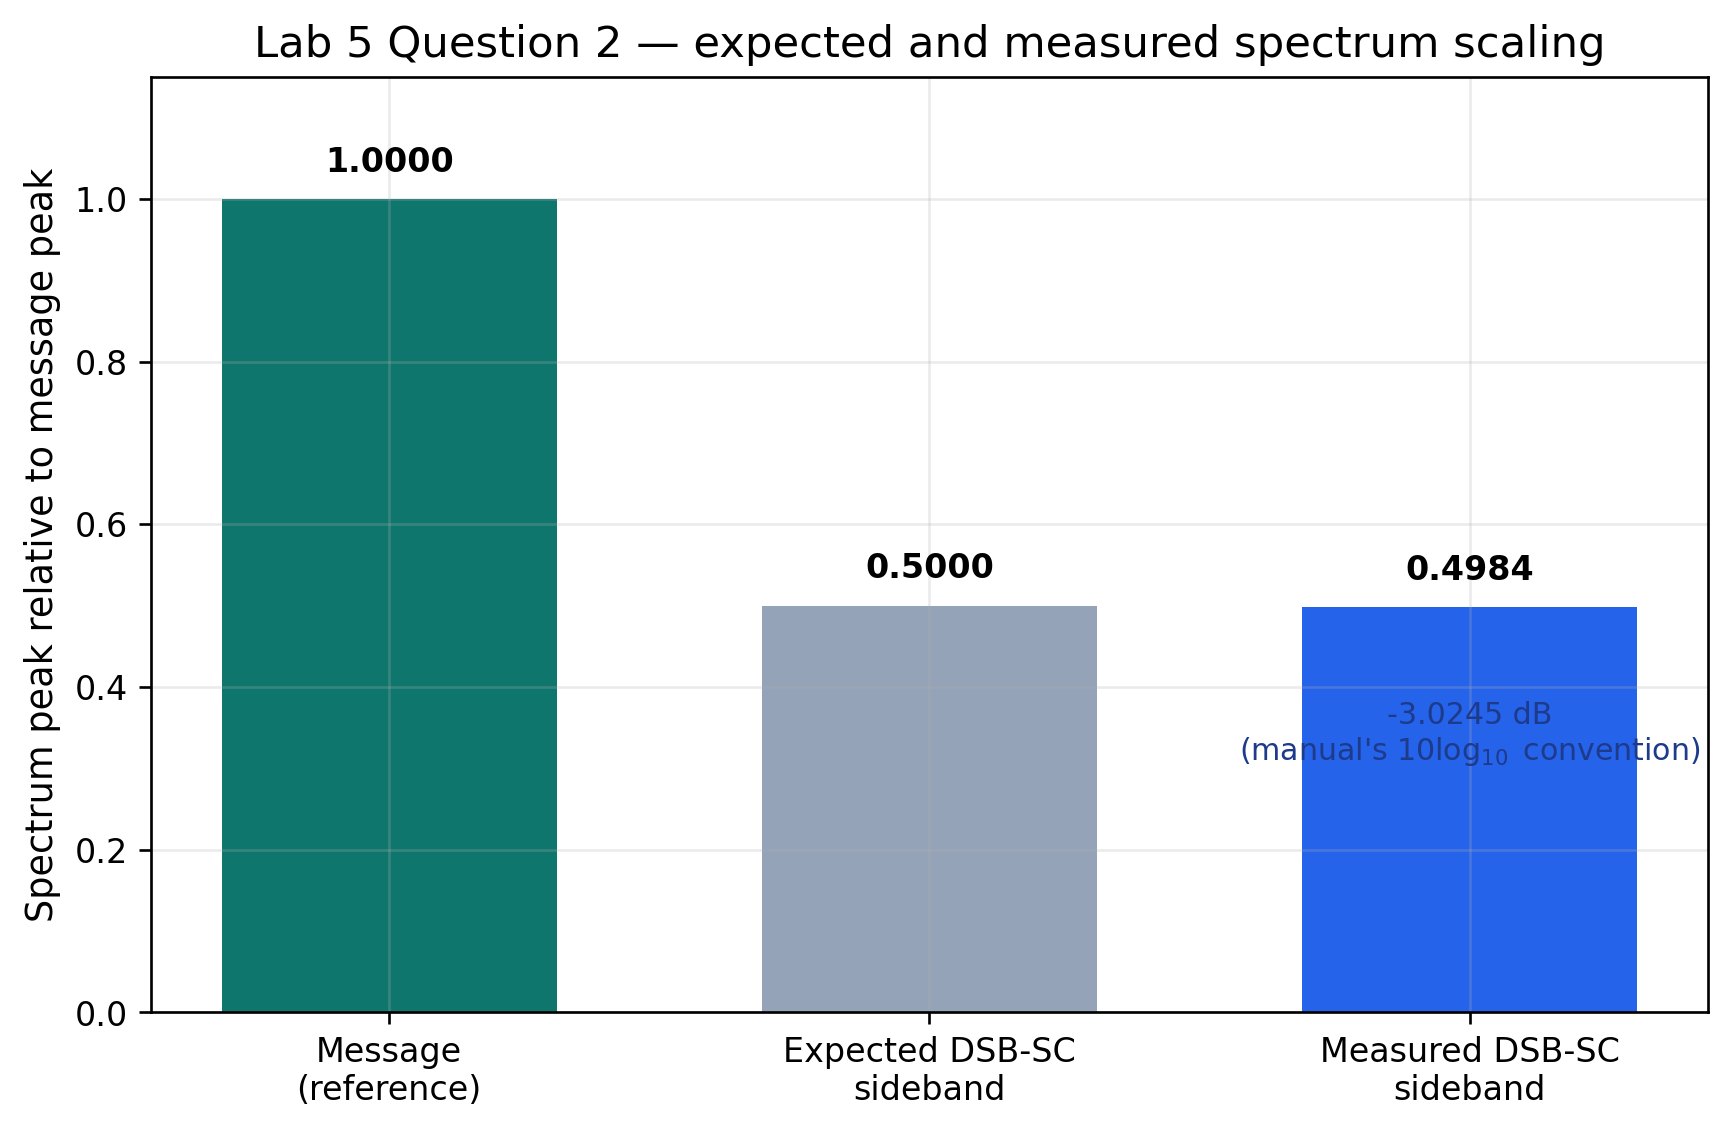
\includegraphics[width=0.88\textwidth]{lab5_q2_scaling.png}
  \caption{Later numerical verification of the Lab 5 Question 2 scaling. This graph supports the interpretation of the in-class spectrum screenshot; it is not presented as a class capture.}
  \label{fig:lab5-scaling}
\end{figure}

\section{My overall reflection}

Lab 4 taught me that understanding the frame structure before recording values was more important than collecting data quickly. With only Nahil and me present, we had to make our process deliberate: identify the correct slots, compare our decoding method with other people, and separate adjustment from recording. The surviving photographs give strong evidence for the equipment, patching and several voltage/code pairs. The graphs also show why I need to preserve raw data honestly: a smooth-looking reconstructed curve would hide the two questionable linear values and the incomplete companded sequence.

Lab 5 showed me that a correct communication-system model still needs disciplined plotting and evidence capture. Our final in-class spectrum screenshot supports the main DSB-SC result, but I did not record the exact decisive plotting edit or save a clearly identified Scope capture. In future labs I will save the final script, the final model, the Scope result, the workspace variables and a short note stating exactly what changed when troubleshooting succeeded.

\begin{checkbox}
The remaining evidence gap is narrow and explicit: I still need the original Lab 4 hardcopy if I want to resolve the $-0.308$ V and $-0.270$ V entries or recover the five missing companded codes. Until then, the raw and partial graphs in this document are the defensible final form of the preserved data.
\end{checkbox}

\end{document}
